\documentclass[twoside]{book}

% Packages required by doxygen
\usepackage{fixltx2e}
\usepackage{calc}
\usepackage{doxygen}
\usepackage[export]{adjustbox} % also loads graphicx
\usepackage{graphicx}
\usepackage[utf8]{inputenc}
\usepackage{makeidx}
\usepackage{multicol}
\usepackage{multirow}
\PassOptionsToPackage{warn}{textcomp}
\usepackage{textcomp}
\usepackage[nointegrals]{wasysym}
\usepackage[table]{xcolor}

% Font selection
\usepackage[T1]{fontenc}
\usepackage[scaled=.90]{helvet}
\usepackage{courier}
\usepackage{amssymb}
\usepackage{sectsty}
\renewcommand{\familydefault}{\sfdefault}
\allsectionsfont{%
  \fontseries{bc}\selectfont%
  \color{darkgray}%
}
\renewcommand{\DoxyLabelFont}{%
  \fontseries{bc}\selectfont%
  \color{darkgray}%
}
\newcommand{\+}{\discretionary{\mbox{\scriptsize$\hookleftarrow$}}{}{}}

% Page & text layout
\usepackage{geometry}
\geometry{%
  a4paper,%
  top=2.5cm,%
  bottom=2.5cm,%
  left=2.5cm,%
  right=2.5cm%
}
\tolerance=750
\hfuzz=15pt
\hbadness=750
\setlength{\emergencystretch}{15pt}
\setlength{\parindent}{0cm}
\setlength{\parskip}{3ex plus 2ex minus 2ex}
\makeatletter
\renewcommand{\paragraph}{%
  \@startsection{paragraph}{4}{0ex}{-1.0ex}{1.0ex}{%
    \normalfont\normalsize\bfseries\SS@parafont%
  }%
}
\renewcommand{\subparagraph}{%
  \@startsection{subparagraph}{5}{0ex}{-1.0ex}{1.0ex}{%
    \normalfont\normalsize\bfseries\SS@subparafont%
  }%
}
\makeatother

% Headers & footers
\usepackage{fancyhdr}
\pagestyle{fancyplain}
\fancyhead[LE]{\fancyplain{}{\bfseries\thepage}}
\fancyhead[CE]{\fancyplain{}{}}
\fancyhead[RE]{\fancyplain{}{\bfseries\leftmark}}
\fancyhead[LO]{\fancyplain{}{\bfseries\rightmark}}
\fancyhead[CO]{\fancyplain{}{}}
\fancyhead[RO]{\fancyplain{}{\bfseries\thepage}}
\fancyfoot[LE]{\fancyplain{}{}}
\fancyfoot[CE]{\fancyplain{}{}}
\fancyfoot[RE]{\fancyplain{}{\bfseries\scriptsize Generated by Doxygen }}
\fancyfoot[LO]{\fancyplain{}{\bfseries\scriptsize Generated by Doxygen }}
\fancyfoot[CO]{\fancyplain{}{}}
\fancyfoot[RO]{\fancyplain{}{}}
\renewcommand{\footrulewidth}{0.4pt}
\renewcommand{\chaptermark}[1]{%
  \markboth{#1}{}%
}
\renewcommand{\sectionmark}[1]{%
  \markright{\thesection\ #1}%
}

% Indices & bibliography
\usepackage{natbib}
\usepackage[titles]{tocloft}
\setcounter{tocdepth}{3}
\setcounter{secnumdepth}{5}
\makeindex

% Hyperlinks (required, but should be loaded last)
\usepackage{ifpdf}
\ifpdf
  \usepackage[pdftex,pagebackref=true]{hyperref}
\else
  \usepackage[ps2pdf,pagebackref=true]{hyperref}
\fi
\hypersetup{%
  colorlinks=true,%
  linkcolor=blue,%
  citecolor=blue,%
  unicode%
}

% Custom commands
\newcommand{\clearemptydoublepage}{%
  \newpage{\pagestyle{empty}\cleardoublepage}%
}

\usepackage{caption}
\captionsetup{labelsep=space,justification=centering,font={bf},singlelinecheck=off,skip=4pt,position=top}

%===== C O N T E N T S =====

\begin{document}

% Titlepage & ToC
\hypersetup{pageanchor=false,
             bookmarksnumbered=true,
             pdfencoding=unicode
            }
\pagenumbering{alph}
\begin{titlepage}
\vspace*{7cm}
\begin{center}%
{\Large Cpp\+Serial\+Port \\[1ex]\large 0.\+0.\+1 }\\
\vspace*{1cm}
{\large Generated by Doxygen 1.8.14}\\
\end{center}
\end{titlepage}
\clearemptydoublepage
\pagenumbering{roman}
\tableofcontents
\clearemptydoublepage
\pagenumbering{arabic}
\hypersetup{pageanchor=true}

%--- Begin generated contents ---
\chapter{Hierarchical Index}
\section{Class Hierarchy}
This inheritance list is sorted roughly, but not completely, alphabetically\+:\begin{DoxyCompactList}
\item \contentsline{section}{Cpp\+Serial\+Port\+:\+:Byte\+Array}{\pageref{class_cpp_serial_port_1_1_byte_array}}{}
\item conditional\+\_\+t\begin{DoxyCompactList}
\item \contentsline{section}{Permuted\+Constructor\+:\+:is\+\_\+included$<$ std\+:\+:tuple$<$ T, Ts... $>$, std\+:\+:tuple$<$ Ts2... $>$ $>$}{\pageref{struct_permuted_constructor_1_1is__included_3_01std_1_1tuple_3_01_t_00_01_ts_8_8_8_01_4_00_01std7773b1cf7a852a22f74d472d1ee753c4}}{}
\end{DoxyCompactList}
\item false\+\_\+type\begin{DoxyCompactList}
\item \contentsline{section}{Permuted\+Constructor\+:\+:has\+\_\+T$<$ T $>$}{\pageref{struct_permuted_constructor_1_1has___t_3_01_t_01_4}}{}
\end{DoxyCompactList}
\item \contentsline{section}{Permuted\+Constructor\+:\+:has\+\_\+T$<$ T, Ts $>$}{\pageref{struct_permuted_constructor_1_1has___t}}{}
\item \contentsline{section}{Permuted\+Constructor\+:\+:has\+\_\+T$<$ T, Ts... $>$}{\pageref{struct_permuted_constructor_1_1has___t}}{}
\begin{DoxyCompactList}
\item \contentsline{section}{Permuted\+Constructor\+:\+:has\+\_\+T$<$ T, Tail, Ts... $>$}{\pageref{struct_permuted_constructor_1_1has___t_3_01_t_00_01_tail_00_01_ts_8_8_8_01_4}}{}
\end{DoxyCompactList}
\item \contentsline{section}{Cpp\+Serial\+Port\+:\+:I\+Byte\+Stream}{\pageref{class_cpp_serial_port_1_1_i_byte_stream}}{}
\begin{DoxyCompactList}
\item \contentsline{section}{Cpp\+Serial\+Port\+:\+:Abstract\+Socket}{\pageref{class_cpp_serial_port_1_1_abstract_socket}}{}
\begin{DoxyCompactList}
\item \contentsline{section}{Cpp\+Serial\+Port\+:\+:Tcp\+Client}{\pageref{class_cpp_serial_port_1_1_tcp_client}}{}
\item \contentsline{section}{Cpp\+Serial\+Port\+:\+:Udp\+Client}{\pageref{class_cpp_serial_port_1_1_udp_client}}{}
\end{DoxyCompactList}
\item \contentsline{section}{Cpp\+Serial\+Port\+:\+:Serial\+Port}{\pageref{class_cpp_serial_port_1_1_serial_port}}{}
\end{DoxyCompactList}
\item \contentsline{section}{Cpp\+Serial\+Port\+:\+:I\+P\+V4\+Address}{\pageref{class_cpp_serial_port_1_1_i_p_v4_address}}{}
\item \contentsline{section}{Permuted\+Constructor\+:\+:is\+\_\+included$<$ T1, T2 $>$}{\pageref{struct_permuted_constructor_1_1is__included}}{}
\item runtime\+\_\+error\begin{DoxyCompactList}
\item \contentsline{section}{Cpp\+Serial\+Port\+:\+:Serial\+Port\+Disconnected\+Exception}{\pageref{class_cpp_serial_port_1_1_serial_port_disconnected_exception}}{}
\item \contentsline{section}{Cpp\+Serial\+Port\+:\+:Socket\+Disconnected\+Exception}{\pageref{class_cpp_serial_port_1_1_socket_disconnected_exception}}{}
\end{DoxyCompactList}
\item true\+\_\+type\begin{DoxyCompactList}
\item \contentsline{section}{Permuted\+Constructor\+:\+:has\+\_\+T$<$ T, T, Ts... $>$}{\pageref{struct_permuted_constructor_1_1has___t_3_01_t_00_01_t_00_01_ts_8_8_8_01_4}}{}
\item \contentsline{section}{Permuted\+Constructor\+:\+:is\+\_\+included$<$ std\+:\+:tuple$<$$>$, std\+:\+:tuple$<$ Ts... $>$ $>$}{\pageref{struct_permuted_constructor_1_1is__included_3_01std_1_1tuple_3_4_00_01std_1_1tuple_3_01_ts_8_8_8_01_4_01_4}}{}
\end{DoxyCompactList}
\item \contentsline{section}{Cpp\+Serial\+Port\+:\+:Underlying\+Bytes}{\pageref{union_cpp_serial_port_1_1_underlying_bytes}}{}
\end{DoxyCompactList}

\chapter{Class Index}
\section{Class List}
Here are the classes, structs, unions and interfaces with brief descriptions\+:\begin{DoxyCompactList}
\item\contentsline{section}{\mbox{\hyperlink{class_cpp_serial_port_1_1_abstract_socket}{Cpp\+Serial\+Port\+::\+Abstract\+Socket}} }{\pageref{class_cpp_serial_port_1_1_abstract_socket}}{}
\item\contentsline{section}{\mbox{\hyperlink{class_cpp_serial_port_1_1_byte_array}{Cpp\+Serial\+Port\+::\+Byte\+Array}} }{\pageref{class_cpp_serial_port_1_1_byte_array}}{}
\item\contentsline{section}{\mbox{\hyperlink{struct_permuted_constructor_1_1has___t}{Permuted\+Constructor\+::has\+\_\+\+T$<$ T, Ts $>$}} }{\pageref{struct_permuted_constructor_1_1has___t}}{}
\item\contentsline{section}{\mbox{\hyperlink{struct_permuted_constructor_1_1has___t_3_01_t_01_4}{Permuted\+Constructor\+::has\+\_\+\+T$<$ T $>$}} }{\pageref{struct_permuted_constructor_1_1has___t_3_01_t_01_4}}{}
\item\contentsline{section}{\mbox{\hyperlink{struct_permuted_constructor_1_1has___t_3_01_t_00_01_t_00_01_ts_8_8_8_01_4}{Permuted\+Constructor\+::has\+\_\+\+T$<$ T, T, Ts... $>$}} }{\pageref{struct_permuted_constructor_1_1has___t_3_01_t_00_01_t_00_01_ts_8_8_8_01_4}}{}
\item\contentsline{section}{\mbox{\hyperlink{struct_permuted_constructor_1_1has___t_3_01_t_00_01_tail_00_01_ts_8_8_8_01_4}{Permuted\+Constructor\+::has\+\_\+\+T$<$ T, Tail, Ts... $>$}} }{\pageref{struct_permuted_constructor_1_1has___t_3_01_t_00_01_tail_00_01_ts_8_8_8_01_4}}{}
\item\contentsline{section}{\mbox{\hyperlink{class_cpp_serial_port_1_1_i_byte_stream}{Cpp\+Serial\+Port\+::\+I\+Byte\+Stream}} }{\pageref{class_cpp_serial_port_1_1_i_byte_stream}}{}
\item\contentsline{section}{\mbox{\hyperlink{class_cpp_serial_port_1_1_i_p_v4_address}{Cpp\+Serial\+Port\+::\+I\+P\+V4\+Address}} }{\pageref{class_cpp_serial_port_1_1_i_p_v4_address}}{}
\item\contentsline{section}{\mbox{\hyperlink{struct_permuted_constructor_1_1is__included}{Permuted\+Constructor\+::is\+\_\+included$<$ T1, T2 $>$}} }{\pageref{struct_permuted_constructor_1_1is__included}}{}
\item\contentsline{section}{\mbox{\hyperlink{struct_permuted_constructor_1_1is__included_3_01std_1_1tuple_3_01_t_00_01_ts_8_8_8_01_4_00_01std7773b1cf7a852a22f74d472d1ee753c4}{Permuted\+Constructor\+::is\+\_\+included$<$ std\+::tuple$<$ T, Ts... $>$, std\+::tuple$<$ Ts2... $>$ $>$}} }{\pageref{struct_permuted_constructor_1_1is__included_3_01std_1_1tuple_3_01_t_00_01_ts_8_8_8_01_4_00_01std7773b1cf7a852a22f74d472d1ee753c4}}{}
\item\contentsline{section}{\mbox{\hyperlink{struct_permuted_constructor_1_1is__included_3_01std_1_1tuple_3_4_00_01std_1_1tuple_3_01_ts_8_8_8_01_4_01_4}{Permuted\+Constructor\+::is\+\_\+included$<$ std\+::tuple$<$$>$, std\+::tuple$<$ Ts... $>$ $>$}} }{\pageref{struct_permuted_constructor_1_1is__included_3_01std_1_1tuple_3_4_00_01std_1_1tuple_3_01_ts_8_8_8_01_4_01_4}}{}
\item\contentsline{section}{\mbox{\hyperlink{class_cpp_serial_port_1_1_serial_port}{Cpp\+Serial\+Port\+::\+Serial\+Port}} }{\pageref{class_cpp_serial_port_1_1_serial_port}}{}
\item\contentsline{section}{\mbox{\hyperlink{class_cpp_serial_port_1_1_serial_port_disconnected_exception}{Cpp\+Serial\+Port\+::\+Serial\+Port\+Disconnected\+Exception}} }{\pageref{class_cpp_serial_port_1_1_serial_port_disconnected_exception}}{}
\item\contentsline{section}{\mbox{\hyperlink{class_cpp_serial_port_1_1_socket_disconnected_exception}{Cpp\+Serial\+Port\+::\+Socket\+Disconnected\+Exception}} }{\pageref{class_cpp_serial_port_1_1_socket_disconnected_exception}}{}
\item\contentsline{section}{\mbox{\hyperlink{class_cpp_serial_port_1_1_tcp_client}{Cpp\+Serial\+Port\+::\+Tcp\+Client}} }{\pageref{class_cpp_serial_port_1_1_tcp_client}}{}
\item\contentsline{section}{\mbox{\hyperlink{class_cpp_serial_port_1_1_udp_client}{Cpp\+Serial\+Port\+::\+Udp\+Client}} }{\pageref{class_cpp_serial_port_1_1_udp_client}}{}
\item\contentsline{section}{\mbox{\hyperlink{union_cpp_serial_port_1_1_underlying_bytes}{Cpp\+Serial\+Port\+::\+Underlying\+Bytes}} }{\pageref{union_cpp_serial_port_1_1_underlying_bytes}}{}
\end{DoxyCompactList}

\chapter{Class Documentation}
\hypertarget{class_cpp_serial_port_1_1_abstract_socket}{}\section{Cpp\+Serial\+Port\+:\+:Abstract\+Socket Class Reference}
\label{class_cpp_serial_port_1_1_abstract_socket}\index{Cpp\+Serial\+Port\+::\+Abstract\+Socket@{Cpp\+Serial\+Port\+::\+Abstract\+Socket}}
Inheritance diagram for Cpp\+Serial\+Port\+:\+:Abstract\+Socket\+:\begin{figure}[H]
\begin{center}
\leavevmode
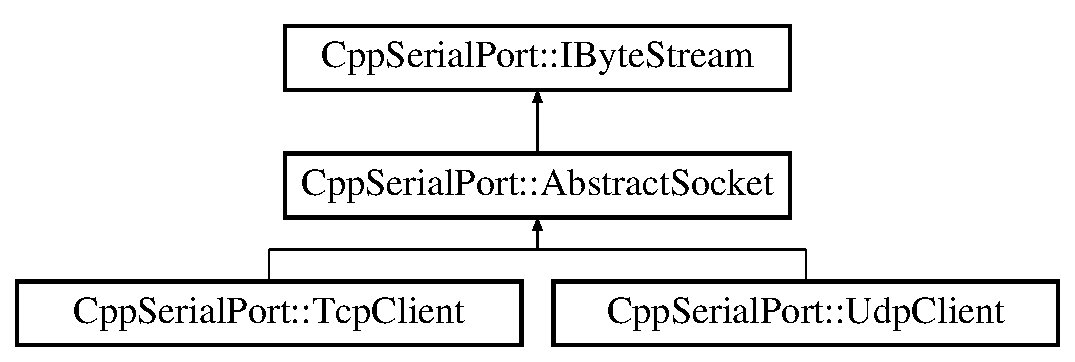
\includegraphics[height=3.000000cm]{class_cpp_serial_port_1_1_abstract_socket}
\end{center}
\end{figure}
\subsection*{Public Member Functions}
\begin{DoxyCompactItemize}
\item 
\mbox{\Hypertarget{class_cpp_serial_port_1_1_abstract_socket_ac3340a5cd4a238884257e01f7127763c}\label{class_cpp_serial_port_1_1_abstract_socket_ac3340a5cd4a238884257e01f7127763c}} 
{\bfseries Abstract\+Socket} (const std\+::string \&host\+Name, uint16\+\_\+t port\+Number)
\item 
\mbox{\Hypertarget{class_cpp_serial_port_1_1_abstract_socket_acc4873d15c4ee4d515900032cede1894}\label{class_cpp_serial_port_1_1_abstract_socket_acc4873d15c4ee4d515900032cede1894}} 
{\bfseries Abstract\+Socket} (const \mbox{\hyperlink{class_cpp_serial_port_1_1_i_p_v4_address}{I\+P\+V4\+Address}} \&ip\+Address, uint16\+\_\+t port\+Number)
\item 
\mbox{\Hypertarget{class_cpp_serial_port_1_1_abstract_socket_abba42cee89e034f7b6639bd801f2dda8}\label{class_cpp_serial_port_1_1_abstract_socket_abba42cee89e034f7b6639bd801f2dda8}} 
ssize\+\_\+t {\bfseries write} (const char $\ast$bytes, size\+\_\+t byte\+Count) override
\item 
\mbox{\Hypertarget{class_cpp_serial_port_1_1_abstract_socket_aff33e9fac306ac5b1d0df9ecb1606e57}\label{class_cpp_serial_port_1_1_abstract_socket_aff33e9fac306ac5b1d0df9ecb1606e57}} 
char {\bfseries read} (bool $\ast$read\+Timeout) override
\item 
\mbox{\Hypertarget{class_cpp_serial_port_1_1_abstract_socket_a13755c32e2e461471598be620043873c}\label{class_cpp_serial_port_1_1_abstract_socket_a13755c32e2e461471598be620043873c}} 
ssize\+\_\+t {\bfseries write} (char i) override
\item 
\mbox{\Hypertarget{class_cpp_serial_port_1_1_abstract_socket_a75e83f0faaad092131daa537b34a2626}\label{class_cpp_serial_port_1_1_abstract_socket_a75e83f0faaad092131daa537b34a2626}} 
std\+::string {\bfseries port\+Name} () const override
\item 
\mbox{\Hypertarget{class_cpp_serial_port_1_1_abstract_socket_abb4b4e7f5a17c0bea04065674a31eb2b}\label{class_cpp_serial_port_1_1_abstract_socket_abb4b4e7f5a17c0bea04065674a31eb2b}} 
bool {\bfseries is\+Open} () const override
\item 
\mbox{\Hypertarget{class_cpp_serial_port_1_1_abstract_socket_a5f23188c33b3e610c263248ad99773a0}\label{class_cpp_serial_port_1_1_abstract_socket_a5f23188c33b3e610c263248ad99773a0}} 
void {\bfseries open\+Port} () override
\item 
\mbox{\Hypertarget{class_cpp_serial_port_1_1_abstract_socket_a8aadacd13b08fc39f964bc57dc3e520d}\label{class_cpp_serial_port_1_1_abstract_socket_a8aadacd13b08fc39f964bc57dc3e520d}} 
void {\bfseries close\+Port} () override
\item 
\mbox{\Hypertarget{class_cpp_serial_port_1_1_abstract_socket_a3270290451ac61f4ed4499d35d28a97c}\label{class_cpp_serial_port_1_1_abstract_socket_a3270290451ac61f4ed4499d35d28a97c}} 
void {\bfseries flush\+Rx} () override
\item 
\mbox{\Hypertarget{class_cpp_serial_port_1_1_abstract_socket_a56c572096cf20273e1a005914f138c9f}\label{class_cpp_serial_port_1_1_abstract_socket_a56c572096cf20273e1a005914f138c9f}} 
void {\bfseries flush\+Tx} () override
\item 
\mbox{\Hypertarget{class_cpp_serial_port_1_1_abstract_socket_a63ed2eb01fb5612329e0d59168eb952e}\label{class_cpp_serial_port_1_1_abstract_socket_a63ed2eb01fb5612329e0d59168eb952e}} 
size\+\_\+t {\bfseries available} () override
\item 
\mbox{\Hypertarget{class_cpp_serial_port_1_1_abstract_socket_a91f8b676933e2e28553fdc2ec9d704c0}\label{class_cpp_serial_port_1_1_abstract_socket_a91f8b676933e2e28553fdc2ec9d704c0}} 
void {\bfseries connect} (const std\+::string \&host\+Name, uint16\+\_\+t port\+Number)
\item 
\mbox{\Hypertarget{class_cpp_serial_port_1_1_abstract_socket_a8598bbc22576ba36d2fb17f959d0b4af}\label{class_cpp_serial_port_1_1_abstract_socket_a8598bbc22576ba36d2fb17f959d0b4af}} 
void {\bfseries connect} ()
\item 
\mbox{\Hypertarget{class_cpp_serial_port_1_1_abstract_socket_a45cb0952ab5cdc8ffe0af83731e2a521}\label{class_cpp_serial_port_1_1_abstract_socket_a45cb0952ab5cdc8ffe0af83731e2a521}} 
bool {\bfseries disconnect} ()
\item 
\mbox{\Hypertarget{class_cpp_serial_port_1_1_abstract_socket_adddb888722410a5c80ca31598d78bdf0}\label{class_cpp_serial_port_1_1_abstract_socket_adddb888722410a5c80ca31598d78bdf0}} 
bool {\bfseries is\+Connected} () const
\item 
\mbox{\Hypertarget{class_cpp_serial_port_1_1_abstract_socket_a8f9e2bab08e06124eb94e853254b0e4b}\label{class_cpp_serial_port_1_1_abstract_socket_a8f9e2bab08e06124eb94e853254b0e4b}} 
void {\bfseries set\+Port\+Number} (uint16\+\_\+t port\+Number)
\item 
\mbox{\Hypertarget{class_cpp_serial_port_1_1_abstract_socket_ac281aef8c2f339f750406b3b45987e9b}\label{class_cpp_serial_port_1_1_abstract_socket_ac281aef8c2f339f750406b3b45987e9b}} 
void {\bfseries set\+Host\+Name} (const std\+::string \&host\+Name)
\item 
\mbox{\Hypertarget{class_cpp_serial_port_1_1_abstract_socket_ad1f6b4e04382235f57d89559f028d7d0}\label{class_cpp_serial_port_1_1_abstract_socket_ad1f6b4e04382235f57d89559f028d7d0}} 
uint16\+\_\+t {\bfseries port\+Number} () const
\item 
\mbox{\Hypertarget{class_cpp_serial_port_1_1_abstract_socket_a30b403222e2b77cc4fd0a2b31d442a08}\label{class_cpp_serial_port_1_1_abstract_socket_a30b403222e2b77cc4fd0a2b31d442a08}} 
std\+::string {\bfseries host\+Name} () const
\end{DoxyCompactItemize}
\subsection*{Static Public Attributes}
\begin{DoxyCompactItemize}
\item 
\mbox{\Hypertarget{class_cpp_serial_port_1_1_abstract_socket_ac4c8c7c03a7c7d08a13f9091cf0c4db2}\label{class_cpp_serial_port_1_1_abstract_socket_ac4c8c7c03a7c7d08a13f9091cf0c4db2}} 
static const uint16\+\_\+t {\bfseries M\+I\+N\+I\+M\+U\+M\+\_\+\+P\+O\+R\+T\+\_\+\+N\+U\+M\+B\+ER} \{1024\}
\item 
\mbox{\Hypertarget{class_cpp_serial_port_1_1_abstract_socket_ae629cbdbf6a2e08eb529ea6e598f61da}\label{class_cpp_serial_port_1_1_abstract_socket_ae629cbdbf6a2e08eb529ea6e598f61da}} 
static const uint16\+\_\+t {\bfseries M\+A\+X\+I\+M\+U\+M\+\_\+\+P\+O\+R\+T\+\_\+\+N\+U\+M\+B\+ER} \{std\+::numeric\+\_\+limits$<$uint16\+\_\+t$>$\+::max()\}
\end{DoxyCompactItemize}
\subsection*{Protected Member Functions}
\begin{DoxyCompactItemize}
\item 
\mbox{\Hypertarget{class_cpp_serial_port_1_1_abstract_socket_a81a8ada743d774b537f77bcee7868cc8}\label{class_cpp_serial_port_1_1_abstract_socket_a81a8ada743d774b537f77bcee7868cc8}} 
virtual ssize\+\_\+t {\bfseries do\+Read} (char $\ast$buffer, size\+\_\+t buffer\+Max)=0
\item 
\mbox{\Hypertarget{class_cpp_serial_port_1_1_abstract_socket_ad617d4ecc652d53cffea1bf1f47579b3}\label{class_cpp_serial_port_1_1_abstract_socket_ad617d4ecc652d53cffea1bf1f47579b3}} 
virtual ssize\+\_\+t {\bfseries do\+Write} (const char $\ast$bytes, size\+\_\+t number\+Of\+Bytes)=0
\item 
\mbox{\Hypertarget{class_cpp_serial_port_1_1_abstract_socket_afff72ec26ca22c4d9bd6c6488b0ec066}\label{class_cpp_serial_port_1_1_abstract_socket_afff72ec26ca22c4d9bd6c6488b0ec066}} 
virtual void {\bfseries do\+Connect} (addrinfo $\ast$address\+Info)=0
\item 
\mbox{\Hypertarget{class_cpp_serial_port_1_1_abstract_socket_a1f57b2412c2ac25a6b3394b7687d9bf6}\label{class_cpp_serial_port_1_1_abstract_socket_a1f57b2412c2ac25a6b3394b7687d9bf6}} 
virtual addrinfo {\bfseries get\+Address\+Info\+Hints} ()=0
\item 
\mbox{\Hypertarget{class_cpp_serial_port_1_1_abstract_socket_a6a8f71f6ce1556c428f44628c19f8161}\label{class_cpp_serial_port_1_1_abstract_socket_a6a8f71f6ce1556c428f44628c19f8161}} 
bool {\bfseries is\+Disconnected} () const
\item 
\mbox{\Hypertarget{class_cpp_serial_port_1_1_abstract_socket_ae1198d2be2aa6033abe0a7f90916a3c6}\label{class_cpp_serial_port_1_1_abstract_socket_ae1198d2be2aa6033abe0a7f90916a3c6}} 
socket\+\_\+t {\bfseries socket\+Descriptor} () const
\item 
\mbox{\Hypertarget{class_cpp_serial_port_1_1_abstract_socket_a9dc9e64a56d7249d982cb074acb723a7}\label{class_cpp_serial_port_1_1_abstract_socket_a9dc9e64a56d7249d982cb074acb723a7}} 
void {\bfseries set\+Socket\+Descriptor} (socket\+\_\+t socket\+Descriptor)
\end{DoxyCompactItemize}
\subsection*{Static Protected Member Functions}
\begin{DoxyCompactItemize}
\item 
\mbox{\Hypertarget{class_cpp_serial_port_1_1_abstract_socket_a077628ef2ab2622d275b79f8ecaba765}\label{class_cpp_serial_port_1_1_abstract_socket_a077628ef2ab2622d275b79f8ecaba765}} 
static timeval {\bfseries to\+Time\+Val} (uint32\+\_\+t total\+Timeout)
\item 
\mbox{\Hypertarget{class_cpp_serial_port_1_1_abstract_socket_a9233ef47772d6c091eb6951b86006f0d}\label{class_cpp_serial_port_1_1_abstract_socket_a9233ef47772d6c091eb6951b86006f0d}} 
static std\+::string {\bfseries get\+Error\+String} (int error\+Code)
\item 
\mbox{\Hypertarget{class_cpp_serial_port_1_1_abstract_socket_a33c329aa73c8358c184c188dd80ddc6e}\label{class_cpp_serial_port_1_1_abstract_socket_a33c329aa73c8358c184c188dd80ddc6e}} 
static int {\bfseries get\+Last\+Error} ()
\end{DoxyCompactItemize}
\subsection*{Additional Inherited Members}


The documentation for this class was generated from the following files\+:\begin{DoxyCompactItemize}
\item 
Cpp\+Serial\+Port/Abstract\+Socket.\+h\item 
Cpp\+Serial\+Port/Abstract\+Socket.\+cpp\end{DoxyCompactItemize}

\hypertarget{class_cpp_serial_port_1_1_byte_array}{}\section{Cpp\+Serial\+Port\+:\+:Byte\+Array Class Reference}
\label{class_cpp_serial_port_1_1_byte_array}\index{Cpp\+Serial\+Port\+::\+Byte\+Array@{Cpp\+Serial\+Port\+::\+Byte\+Array}}
\subsection*{Public Member Functions}
\begin{DoxyCompactItemize}
\item 
\mbox{\Hypertarget{class_cpp_serial_port_1_1_byte_array_a3835532697d7ef23ce67c5c700a0cb79}\label{class_cpp_serial_port_1_1_byte_array_a3835532697d7ef23ce67c5c700a0cb79}} 
{\bfseries Byte\+Array} (char c)
\item 
\mbox{\Hypertarget{class_cpp_serial_port_1_1_byte_array_a3ceb66dbb01620ca3836dbbe931284dd}\label{class_cpp_serial_port_1_1_byte_array_a3ceb66dbb01620ca3836dbbe931284dd}} 
{\bfseries Byte\+Array} (const char $\ast$c\+Str)
\item 
\mbox{\Hypertarget{class_cpp_serial_port_1_1_byte_array_a3883ddeeadd56c022052d33315e07e01}\label{class_cpp_serial_port_1_1_byte_array_a3883ddeeadd56c022052d33315e07e01}} 
{\bfseries Byte\+Array} (const std\+::string \&str)
\item 
\mbox{\Hypertarget{class_cpp_serial_port_1_1_byte_array_a8665a2be617f7069530f8c9791b19b4f}\label{class_cpp_serial_port_1_1_byte_array_a8665a2be617f7069530f8c9791b19b4f}} 
{\bfseries Byte\+Array} (char $\ast$buffer, size\+\_\+t length)
\item 
\mbox{\Hypertarget{class_cpp_serial_port_1_1_byte_array_af07ee95b3a54ec839bbea1fa8a6f3d0e}\label{class_cpp_serial_port_1_1_byte_array_af07ee95b3a54ec839bbea1fa8a6f3d0e}} 
{\bfseries Byte\+Array} (const std\+::vector$<$ char $>$ \&byte\+Array)
\item 
\mbox{\Hypertarget{class_cpp_serial_port_1_1_byte_array_a46fe561f131958df56257d94b2ea6436}\label{class_cpp_serial_port_1_1_byte_array_a46fe561f131958df56257d94b2ea6436}} 
\mbox{\hyperlink{class_cpp_serial_port_1_1_byte_array}{Byte\+Array}} \& {\bfseries operator=} (const \mbox{\hyperlink{class_cpp_serial_port_1_1_byte_array}{Byte\+Array}} \&rhs)
\item 
\mbox{\Hypertarget{class_cpp_serial_port_1_1_byte_array_ac225b1ab9472ad2d6be54b9c402750b6}\label{class_cpp_serial_port_1_1_byte_array_ac225b1ab9472ad2d6be54b9c402750b6}} 
\mbox{\hyperlink{class_cpp_serial_port_1_1_byte_array}{Byte\+Array}} \& {\bfseries operator=} (const std\+::vector$<$ char $>$ \&rhs)
\item 
\mbox{\Hypertarget{class_cpp_serial_port_1_1_byte_array_ae19a4bc286a8e5f4f70e2cc2bb54d94e}\label{class_cpp_serial_port_1_1_byte_array_ae19a4bc286a8e5f4f70e2cc2bb54d94e}} 
\mbox{\hyperlink{class_cpp_serial_port_1_1_byte_array}{Byte\+Array}} \& {\bfseries operator=} (const std\+::string \&rhs)
\item 
\mbox{\Hypertarget{class_cpp_serial_port_1_1_byte_array_ac47b9704fc6b80017c55a5f8d5c52add}\label{class_cpp_serial_port_1_1_byte_array_ac47b9704fc6b80017c55a5f8d5c52add}} 
\mbox{\hyperlink{class_cpp_serial_port_1_1_byte_array}{Byte\+Array}} \& {\bfseries operator=} (char c)
\item 
\mbox{\Hypertarget{class_cpp_serial_port_1_1_byte_array_a1d673ed2c949891a97f4333d94bdbe4f}\label{class_cpp_serial_port_1_1_byte_array_a1d673ed2c949891a97f4333d94bdbe4f}} 
\mbox{\hyperlink{class_cpp_serial_port_1_1_byte_array}{Byte\+Array}} \& {\bfseries operator=} (\mbox{\hyperlink{class_cpp_serial_port_1_1_byte_array}{Byte\+Array}} \&\&rhs)
\item 
\mbox{\Hypertarget{class_cpp_serial_port_1_1_byte_array_a82f7485c157ed475cf66d6a21f418a26}\label{class_cpp_serial_port_1_1_byte_array_a82f7485c157ed475cf66d6a21f418a26}} 
\mbox{\hyperlink{class_cpp_serial_port_1_1_byte_array}{Byte\+Array}} \& {\bfseries operator=} (std\+::vector$<$ char $>$ \&\&rhs)
\item 
\mbox{\Hypertarget{class_cpp_serial_port_1_1_byte_array_a741295aadad88940dd55b198705fa2b4}\label{class_cpp_serial_port_1_1_byte_array_a741295aadad88940dd55b198705fa2b4}} 
{\bfseries Byte\+Array} (const \mbox{\hyperlink{class_cpp_serial_port_1_1_byte_array}{Byte\+Array}} \&other)=default
\item 
\mbox{\Hypertarget{class_cpp_serial_port_1_1_byte_array_ac62463175704a7f008f65ab74026d59e}\label{class_cpp_serial_port_1_1_byte_array_ac62463175704a7f008f65ab74026d59e}} 
{\bfseries Byte\+Array} (\mbox{\hyperlink{class_cpp_serial_port_1_1_byte_array}{Byte\+Array}} \&\&other)=default
\item 
\mbox{\Hypertarget{class_cpp_serial_port_1_1_byte_array_a52ec9a47a2c27ae920c79a898c6ff0b7}\label{class_cpp_serial_port_1_1_byte_array_a52ec9a47a2c27ae920c79a898c6ff0b7}} 
{\footnotesize template$<$typename Input\+Iterator $>$ }\\{\bfseries Byte\+Array} (Input\+Iterator begin, Input\+Iterator end)
\item 
\mbox{\Hypertarget{class_cpp_serial_port_1_1_byte_array_a98f2a03187ba0776f174ac9aaa9a9fd1}\label{class_cpp_serial_port_1_1_byte_array_a98f2a03187ba0776f174ac9aaa9a9fd1}} 
\mbox{\hyperlink{class_cpp_serial_port_1_1_byte_array}{Byte\+Array}} \& {\bfseries append} (char c)
\item 
\mbox{\Hypertarget{class_cpp_serial_port_1_1_byte_array_a790911e3d14b042d6fdae1b8939c8c43}\label{class_cpp_serial_port_1_1_byte_array_a790911e3d14b042d6fdae1b8939c8c43}} 
\mbox{\hyperlink{class_cpp_serial_port_1_1_byte_array}{Byte\+Array}} \& {\bfseries append} (const \mbox{\hyperlink{class_cpp_serial_port_1_1_byte_array}{Byte\+Array}} \&rhs)
\item 
\mbox{\Hypertarget{class_cpp_serial_port_1_1_byte_array_a470d0279633178bf956a3243d3eb8ad4}\label{class_cpp_serial_port_1_1_byte_array_a470d0279633178bf956a3243d3eb8ad4}} 
\mbox{\hyperlink{class_cpp_serial_port_1_1_byte_array}{Byte\+Array}} \& {\bfseries append} (const std\+::string \&rhs)
\item 
\mbox{\Hypertarget{class_cpp_serial_port_1_1_byte_array_a2a9b3fb214fd753fc58041b2d9c35742}\label{class_cpp_serial_port_1_1_byte_array_a2a9b3fb214fd753fc58041b2d9c35742}} 
\mbox{\hyperlink{class_cpp_serial_port_1_1_byte_array}{Byte\+Array}} \& {\bfseries append} (const std\+::vector$<$ char $>$ \&rhs)
\item 
\mbox{\Hypertarget{class_cpp_serial_port_1_1_byte_array_afc700484f1a4bb8ebffe6b5c80f1585c}\label{class_cpp_serial_port_1_1_byte_array_afc700484f1a4bb8ebffe6b5c80f1585c}} 
\mbox{\hyperlink{class_cpp_serial_port_1_1_byte_array}{Byte\+Array}} \& {\bfseries operator+=} (char c)
\item 
\mbox{\Hypertarget{class_cpp_serial_port_1_1_byte_array_a7a1995916b8439b46aa0d36ef38ef7c0}\label{class_cpp_serial_port_1_1_byte_array_a7a1995916b8439b46aa0d36ef38ef7c0}} 
\mbox{\hyperlink{class_cpp_serial_port_1_1_byte_array}{Byte\+Array}} \& {\bfseries operator+=} (const \mbox{\hyperlink{class_cpp_serial_port_1_1_byte_array}{Byte\+Array}} \&rhs)
\item 
\mbox{\Hypertarget{class_cpp_serial_port_1_1_byte_array_a12aa808a8e9eda49a86cc7143cc789e6}\label{class_cpp_serial_port_1_1_byte_array_a12aa808a8e9eda49a86cc7143cc789e6}} 
\mbox{\hyperlink{class_cpp_serial_port_1_1_byte_array}{Byte\+Array}} \& {\bfseries operator+=} (const std\+::string \&rhs)
\item 
\mbox{\Hypertarget{class_cpp_serial_port_1_1_byte_array_a0bc3c9d2563ba6bceea3f0be9710b079}\label{class_cpp_serial_port_1_1_byte_array_a0bc3c9d2563ba6bceea3f0be9710b079}} 
\mbox{\hyperlink{class_cpp_serial_port_1_1_byte_array}{Byte\+Array}} \& {\bfseries operator+=} (const std\+::vector$<$ char $>$ \&rhs)
\item 
\mbox{\Hypertarget{class_cpp_serial_port_1_1_byte_array_a39f7aafe01f4820efcf8c8ff3f96d0f2}\label{class_cpp_serial_port_1_1_byte_array_a39f7aafe01f4820efcf8c8ff3f96d0f2}} 
\mbox{\hyperlink{class_cpp_serial_port_1_1_byte_array}{Byte\+Array}} \& {\bfseries operator+} (char c)
\item 
\mbox{\Hypertarget{class_cpp_serial_port_1_1_byte_array_ac5efe720d49ff50a9538385236010744}\label{class_cpp_serial_port_1_1_byte_array_ac5efe720d49ff50a9538385236010744}} 
\mbox{\hyperlink{class_cpp_serial_port_1_1_byte_array}{Byte\+Array}} \& {\bfseries operator+} (const \mbox{\hyperlink{class_cpp_serial_port_1_1_byte_array}{Byte\+Array}} \&rhs)
\item 
\mbox{\Hypertarget{class_cpp_serial_port_1_1_byte_array_a4fbd9e26d0671a4737fa652c3719a4ee}\label{class_cpp_serial_port_1_1_byte_array_a4fbd9e26d0671a4737fa652c3719a4ee}} 
\mbox{\hyperlink{class_cpp_serial_port_1_1_byte_array}{Byte\+Array}} \& {\bfseries operator+} (const std\+::string \&rhs)
\item 
\mbox{\Hypertarget{class_cpp_serial_port_1_1_byte_array_af2da5468dde68c869a4037923292c1ab}\label{class_cpp_serial_port_1_1_byte_array_af2da5468dde68c869a4037923292c1ab}} 
\mbox{\hyperlink{class_cpp_serial_port_1_1_byte_array}{Byte\+Array}} \& {\bfseries operator+} (const std\+::vector$<$ char $>$ \&rhs)
\item 
\mbox{\Hypertarget{class_cpp_serial_port_1_1_byte_array_a8065fa7a92390e122d34ebc49c6cf6d5}\label{class_cpp_serial_port_1_1_byte_array_a8065fa7a92390e122d34ebc49c6cf6d5}} 
size\+\_\+t {\bfseries find} (const \mbox{\hyperlink{class_cpp_serial_port_1_1_byte_array}{Byte\+Array}} \&to\+Find)
\item 
\mbox{\Hypertarget{class_cpp_serial_port_1_1_byte_array_ad2f25aae1da2bbf4544ddd3d25bd8513}\label{class_cpp_serial_port_1_1_byte_array_ad2f25aae1da2bbf4544ddd3d25bd8513}} 
size\+\_\+t {\bfseries find} (char c)
\item 
\mbox{\Hypertarget{class_cpp_serial_port_1_1_byte_array_a647c1192a45b6307d1f19177b8408354}\label{class_cpp_serial_port_1_1_byte_array_a647c1192a45b6307d1f19177b8408354}} 
std\+::vector$<$ char $>$\+::iterator {\bfseries begin} ()
\item 
\mbox{\Hypertarget{class_cpp_serial_port_1_1_byte_array_adbc9bf23f4acbfd80e846c0102b82808}\label{class_cpp_serial_port_1_1_byte_array_adbc9bf23f4acbfd80e846c0102b82808}} 
const std\+::vector$<$ char $>$\+::const\+\_\+iterator {\bfseries cbegin} () const
\item 
\mbox{\Hypertarget{class_cpp_serial_port_1_1_byte_array_a7531a1636f7309e7e3071b03f0a4c3ec}\label{class_cpp_serial_port_1_1_byte_array_a7531a1636f7309e7e3071b03f0a4c3ec}} 
std\+::vector$<$ char $>$\+::reverse\+\_\+iterator {\bfseries rbegin} ()
\item 
\mbox{\Hypertarget{class_cpp_serial_port_1_1_byte_array_a6b5a1909626fd69bb0b7b1edddbdc305}\label{class_cpp_serial_port_1_1_byte_array_a6b5a1909626fd69bb0b7b1edddbdc305}} 
const std\+::vector$<$ char $>$\+::const\+\_\+reverse\+\_\+iterator {\bfseries crbegin} () const
\item 
\mbox{\Hypertarget{class_cpp_serial_port_1_1_byte_array_a7ec886b5df3959bd609533371c5f35eb}\label{class_cpp_serial_port_1_1_byte_array_a7ec886b5df3959bd609533371c5f35eb}} 
std\+::vector$<$ char $>$\+::iterator {\bfseries end} ()
\item 
\mbox{\Hypertarget{class_cpp_serial_port_1_1_byte_array_a108876f39ce7301ffc80d166f7e06d16}\label{class_cpp_serial_port_1_1_byte_array_a108876f39ce7301ffc80d166f7e06d16}} 
const std\+::vector$<$ char $>$\+::const\+\_\+iterator {\bfseries cend} () const
\item 
\mbox{\Hypertarget{class_cpp_serial_port_1_1_byte_array_abe2f611dfdc320573e10f171a87f01a8}\label{class_cpp_serial_port_1_1_byte_array_abe2f611dfdc320573e10f171a87f01a8}} 
std\+::vector$<$ char $>$\+::reverse\+\_\+iterator {\bfseries rend} ()
\item 
\mbox{\Hypertarget{class_cpp_serial_port_1_1_byte_array_a0dafa827bdea28dad5c10f7d69983a92}\label{class_cpp_serial_port_1_1_byte_array_a0dafa827bdea28dad5c10f7d69983a92}} 
const std\+::vector$<$ char $>$\+::const\+\_\+reverse\+\_\+iterator {\bfseries crend} () const
\item 
\mbox{\Hypertarget{class_cpp_serial_port_1_1_byte_array_a48bf7d4cd12c3702918025afb54a2f3e}\label{class_cpp_serial_port_1_1_byte_array_a48bf7d4cd12c3702918025afb54a2f3e}} 
\mbox{\hyperlink{class_cpp_serial_port_1_1_byte_array}{Byte\+Array}} \& {\bfseries clear} ()
\item 
\mbox{\Hypertarget{class_cpp_serial_port_1_1_byte_array_a189aeb360394d6c2126252f34c3e182b}\label{class_cpp_serial_port_1_1_byte_array_a189aeb360394d6c2126252f34c3e182b}} 
size\+\_\+t {\bfseries size} () const
\item 
\mbox{\Hypertarget{class_cpp_serial_port_1_1_byte_array_adb5d869f9cdf24ea28a02a03e714159b}\label{class_cpp_serial_port_1_1_byte_array_adb5d869f9cdf24ea28a02a03e714159b}} 
size\+\_\+t {\bfseries length} () const
\item 
\mbox{\Hypertarget{class_cpp_serial_port_1_1_byte_array_a9684151c301594c21c41b981d0eb8675}\label{class_cpp_serial_port_1_1_byte_array_a9684151c301594c21c41b981d0eb8675}} 
bool {\bfseries empty} () const
\item 
\mbox{\Hypertarget{class_cpp_serial_port_1_1_byte_array_ae7b0802ee7fb4cbd620c1daf39d0f7b3}\label{class_cpp_serial_port_1_1_byte_array_ae7b0802ee7fb4cbd620c1daf39d0f7b3}} 
const char $\ast$ {\bfseries data} () const
\item 
\mbox{\Hypertarget{class_cpp_serial_port_1_1_byte_array_ab4fe8ef1a4f769c2e967da2a96aed424}\label{class_cpp_serial_port_1_1_byte_array_ab4fe8ef1a4f769c2e967da2a96aed424}} 
char $\ast$ {\bfseries data} ()
\item 
\mbox{\Hypertarget{class_cpp_serial_port_1_1_byte_array_a5bb45a1237fdc9d601a523c44bc2ae65}\label{class_cpp_serial_port_1_1_byte_array_a5bb45a1237fdc9d601a523c44bc2ae65}} 
\mbox{\hyperlink{class_cpp_serial_port_1_1_byte_array}{Byte\+Array}} \& {\bfseries pop\+Back} ()
\item 
\mbox{\Hypertarget{class_cpp_serial_port_1_1_byte_array_a3cb1a6536851dad97d16affd7fd5147a}\label{class_cpp_serial_port_1_1_byte_array_a3cb1a6536851dad97d16affd7fd5147a}} 
\mbox{\hyperlink{class_cpp_serial_port_1_1_byte_array}{Byte\+Array}} \& {\bfseries pop\+Front} ()
\item 
\mbox{\Hypertarget{class_cpp_serial_port_1_1_byte_array_a5c001fee989607b6a015d8444757828c}\label{class_cpp_serial_port_1_1_byte_array_a5c001fee989607b6a015d8444757828c}} 
char \& {\bfseries operator\mbox{[}$\,$\mbox{]}} (size\+\_\+t index)
\item 
\mbox{\Hypertarget{class_cpp_serial_port_1_1_byte_array_a2007c2a088746dab7292362a2997d875}\label{class_cpp_serial_port_1_1_byte_array_a2007c2a088746dab7292362a2997d875}} 
const char \& {\bfseries operator\mbox{[}$\,$\mbox{]}} (size\+\_\+t index) const
\item 
\mbox{\Hypertarget{class_cpp_serial_port_1_1_byte_array_a6f0578b010cb1aae46e30bebd276922b}\label{class_cpp_serial_port_1_1_byte_array_a6f0578b010cb1aae46e30bebd276922b}} 
char \& {\bfseries at} (size\+\_\+t index)
\item 
\mbox{\Hypertarget{class_cpp_serial_port_1_1_byte_array_a937d64f4f1e51da7927e6e9a6974c7e9}\label{class_cpp_serial_port_1_1_byte_array_a937d64f4f1e51da7927e6e9a6974c7e9}} 
const char \& {\bfseries at} (size\+\_\+t index) const
\item 
\mbox{\Hypertarget{class_cpp_serial_port_1_1_byte_array_ae5ffac67be63d8460bab8629a3b8abf1}\label{class_cpp_serial_port_1_1_byte_array_ae5ffac67be63d8460bab8629a3b8abf1}} 
\mbox{\hyperlink{class_cpp_serial_port_1_1_byte_array}{Byte\+Array}} {\bfseries subsequence} (size\+\_\+t index, size\+\_\+t length=0) const
\item 
\mbox{\Hypertarget{class_cpp_serial_port_1_1_byte_array_a3d166620e56a10cae5fdca7146049df3}\label{class_cpp_serial_port_1_1_byte_array_a3d166620e56a10cae5fdca7146049df3}} 
{\bfseries operator std\+::string} () const
\item 
\mbox{\Hypertarget{class_cpp_serial_port_1_1_byte_array_a306587c32700189c63b87c74ee545e88}\label{class_cpp_serial_port_1_1_byte_array_a306587c32700189c63b87c74ee545e88}} 
std\+::string {\bfseries to\+String} () const
\item 
\mbox{\Hypertarget{class_cpp_serial_port_1_1_byte_array_a17d02a928f65365caafefe734bd4eb11}\label{class_cpp_serial_port_1_1_byte_array_a17d02a928f65365caafefe734bd4eb11}} 
bool {\bfseries ends\+With} (char $\ast$buffer, size\+\_\+t length) const
\item 
\mbox{\Hypertarget{class_cpp_serial_port_1_1_byte_array_acee5d5286d1cd52df13e4a365dac296c}\label{class_cpp_serial_port_1_1_byte_array_acee5d5286d1cd52df13e4a365dac296c}} 
bool {\bfseries ends\+With} (const char $\ast$c\+Str) const
\item 
\mbox{\Hypertarget{class_cpp_serial_port_1_1_byte_array_af42e1ee52db0628f0370f53e1331da8b}\label{class_cpp_serial_port_1_1_byte_array_af42e1ee52db0628f0370f53e1331da8b}} 
bool {\bfseries ends\+With} (const std\+::string \&str) const
\item 
\mbox{\Hypertarget{class_cpp_serial_port_1_1_byte_array_af2184794bed19453f35de421ce73157b}\label{class_cpp_serial_port_1_1_byte_array_af2184794bed19453f35de421ce73157b}} 
bool {\bfseries ends\+With} (const \mbox{\hyperlink{class_cpp_serial_port_1_1_byte_array}{Byte\+Array}} \&byte\+Array) const
\item 
\mbox{\Hypertarget{class_cpp_serial_port_1_1_byte_array_a17a744f091521f48097efe35a0e10d2e}\label{class_cpp_serial_port_1_1_byte_array_a17a744f091521f48097efe35a0e10d2e}} 
bool {\bfseries starts\+With} (const \mbox{\hyperlink{class_cpp_serial_port_1_1_byte_array}{Byte\+Array}} \&byte\+Array) const
\item 
\mbox{\Hypertarget{class_cpp_serial_port_1_1_byte_array_accc312c1828fda5f2109084be0c2649b}\label{class_cpp_serial_port_1_1_byte_array_accc312c1828fda5f2109084be0c2649b}} 
bool {\bfseries starts\+With} (char $\ast$buffer, size\+\_\+t length) const
\item 
\mbox{\Hypertarget{class_cpp_serial_port_1_1_byte_array_ad5a9365f8a12bdbd2f626d7ba6f70b96}\label{class_cpp_serial_port_1_1_byte_array_ad5a9365f8a12bdbd2f626d7ba6f70b96}} 
bool {\bfseries starts\+With} (const char $\ast$c\+Str) const
\item 
\mbox{\Hypertarget{class_cpp_serial_port_1_1_byte_array_a488dace2577458a9948c13745a5f4722}\label{class_cpp_serial_port_1_1_byte_array_a488dace2577458a9948c13745a5f4722}} 
bool {\bfseries starts\+With} (const std\+::string \&str) const
\end{DoxyCompactItemize}
\subsection*{Friends}
\begin{DoxyCompactItemize}
\item 
\mbox{\Hypertarget{class_cpp_serial_port_1_1_byte_array_a76332659506cc3c3ecaec0d305c59de9}\label{class_cpp_serial_port_1_1_byte_array_a76332659506cc3c3ecaec0d305c59de9}} 
\mbox{\hyperlink{class_cpp_serial_port_1_1_byte_array}{Byte\+Array}} {\bfseries operator+} (char c, const \mbox{\hyperlink{class_cpp_serial_port_1_1_byte_array}{Byte\+Array}} \&rhs)
\item 
\mbox{\Hypertarget{class_cpp_serial_port_1_1_byte_array_a35b059cbb7652131e2e9a8151ad67db3}\label{class_cpp_serial_port_1_1_byte_array_a35b059cbb7652131e2e9a8151ad67db3}} 
\mbox{\hyperlink{class_cpp_serial_port_1_1_byte_array}{Byte\+Array}} {\bfseries operator+} (const \mbox{\hyperlink{class_cpp_serial_port_1_1_byte_array}{Byte\+Array}} \&lhs, const \mbox{\hyperlink{class_cpp_serial_port_1_1_byte_array}{Byte\+Array}} \&rhs)
\item 
\mbox{\Hypertarget{class_cpp_serial_port_1_1_byte_array_a72b61cc5ade4da63abce18c96b18c9f1}\label{class_cpp_serial_port_1_1_byte_array_a72b61cc5ade4da63abce18c96b18c9f1}} 
\mbox{\hyperlink{class_cpp_serial_port_1_1_byte_array}{Byte\+Array}} {\bfseries operator+} (const std\+::string \&lhs, const \mbox{\hyperlink{class_cpp_serial_port_1_1_byte_array}{Byte\+Array}} \&rhs)
\item 
\mbox{\Hypertarget{class_cpp_serial_port_1_1_byte_array_af5fb63acc032e53e7c336ba7fb64229e}\label{class_cpp_serial_port_1_1_byte_array_af5fb63acc032e53e7c336ba7fb64229e}} 
\mbox{\hyperlink{class_cpp_serial_port_1_1_byte_array}{Byte\+Array}} {\bfseries operator+} (const std\+::vector$<$ char $>$ \&lhs, const \mbox{\hyperlink{class_cpp_serial_port_1_1_byte_array}{Byte\+Array}} \&rhs)
\item 
\mbox{\Hypertarget{class_cpp_serial_port_1_1_byte_array_a3766c56e8a8886283657da1df994a7a4}\label{class_cpp_serial_port_1_1_byte_array_a3766c56e8a8886283657da1df994a7a4}} 
\mbox{\hyperlink{class_cpp_serial_port_1_1_byte_array}{Byte\+Array}} {\bfseries operator+} (const \mbox{\hyperlink{class_cpp_serial_port_1_1_byte_array}{Byte\+Array}} \&lhs, char c)
\item 
\mbox{\Hypertarget{class_cpp_serial_port_1_1_byte_array_a9f8c740a46266a3deb922e3fc0dcee37}\label{class_cpp_serial_port_1_1_byte_array_a9f8c740a46266a3deb922e3fc0dcee37}} 
\mbox{\hyperlink{class_cpp_serial_port_1_1_byte_array}{Byte\+Array}} {\bfseries operator+} (const \mbox{\hyperlink{class_cpp_serial_port_1_1_byte_array}{Byte\+Array}} \&lhs, const std\+::string \&rhs)
\item 
\mbox{\Hypertarget{class_cpp_serial_port_1_1_byte_array_acb065e9e57edc2b4c1b4c2831dea38bd}\label{class_cpp_serial_port_1_1_byte_array_acb065e9e57edc2b4c1b4c2831dea38bd}} 
\mbox{\hyperlink{class_cpp_serial_port_1_1_byte_array}{Byte\+Array}} {\bfseries operator+} (const \mbox{\hyperlink{class_cpp_serial_port_1_1_byte_array}{Byte\+Array}} \&lhs, const std\+::vector$<$ char $>$ \&rhs)
\item 
\mbox{\Hypertarget{class_cpp_serial_port_1_1_byte_array_aef2aa19830496269553a5f508f0225de}\label{class_cpp_serial_port_1_1_byte_array_aef2aa19830496269553a5f508f0225de}} 
bool {\bfseries operator==} (const \mbox{\hyperlink{class_cpp_serial_port_1_1_byte_array}{Byte\+Array}} \&lhs, const \mbox{\hyperlink{class_cpp_serial_port_1_1_byte_array}{Byte\+Array}} \&rhs)
\end{DoxyCompactItemize}


The documentation for this class was generated from the following files\+:\begin{DoxyCompactItemize}
\item 
Cpp\+Serial\+Port/Byte\+Array.\+h\item 
Cpp\+Serial\+Port/Byte\+Array.\+cpp\end{DoxyCompactItemize}

\hypertarget{struct_permuted_constructor_1_1has___t}{}\section{Permuted\+Constructor\+:\+:has\+\_\+T$<$ T, Ts $>$ Struct Template Reference}
\label{struct_permuted_constructor_1_1has___t}\index{Permuted\+Constructor\+::has\+\_\+\+T$<$ T, Ts $>$@{Permuted\+Constructor\+::has\+\_\+\+T$<$ T, Ts $>$}}


The documentation for this struct was generated from the following file\+:\begin{DoxyCompactItemize}
\item 
Cpp\+Serial\+Port/Serial\+Port.\+h\end{DoxyCompactItemize}

\hypertarget{struct_permuted_constructor_1_1has___t_3_01_t_01_4}{}\section{Permuted\+Constructor\+:\+:has\+\_\+T$<$ T $>$ Struct Template Reference}
\label{struct_permuted_constructor_1_1has___t_3_01_t_01_4}\index{Permuted\+Constructor\+::has\+\_\+\+T$<$ T $>$@{Permuted\+Constructor\+::has\+\_\+\+T$<$ T $>$}}
Inheritance diagram for Permuted\+Constructor\+:\+:has\+\_\+T$<$ T $>$\+:\begin{figure}[H]
\begin{center}
\leavevmode
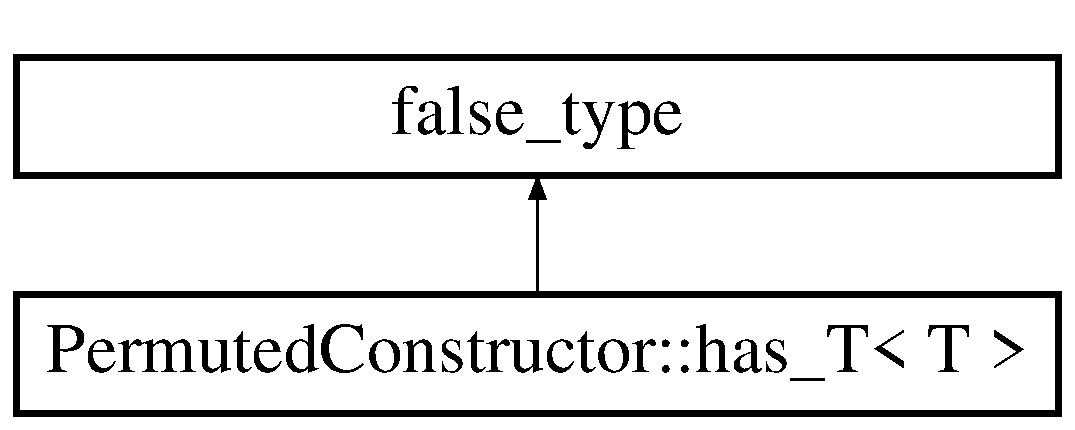
\includegraphics[height=2.000000cm]{struct_permuted_constructor_1_1has___t_3_01_t_01_4}
\end{center}
\end{figure}


The documentation for this struct was generated from the following file\+:\begin{DoxyCompactItemize}
\item 
Cpp\+Serial\+Port/Serial\+Port.\+h\end{DoxyCompactItemize}

\hypertarget{struct_permuted_constructor_1_1has___t_3_01_t_00_01_t_00_01_ts_8_8_8_01_4}{}\section{Permuted\+Constructor\+:\+:has\+\_\+T$<$ T, T, Ts... $>$ Struct Template Reference}
\label{struct_permuted_constructor_1_1has___t_3_01_t_00_01_t_00_01_ts_8_8_8_01_4}\index{Permuted\+Constructor\+::has\+\_\+\+T$<$ T, T, Ts... $>$@{Permuted\+Constructor\+::has\+\_\+\+T$<$ T, T, Ts... $>$}}
Inheritance diagram for Permuted\+Constructor\+:\+:has\+\_\+T$<$ T, T, Ts... $>$\+:\begin{figure}[H]
\begin{center}
\leavevmode
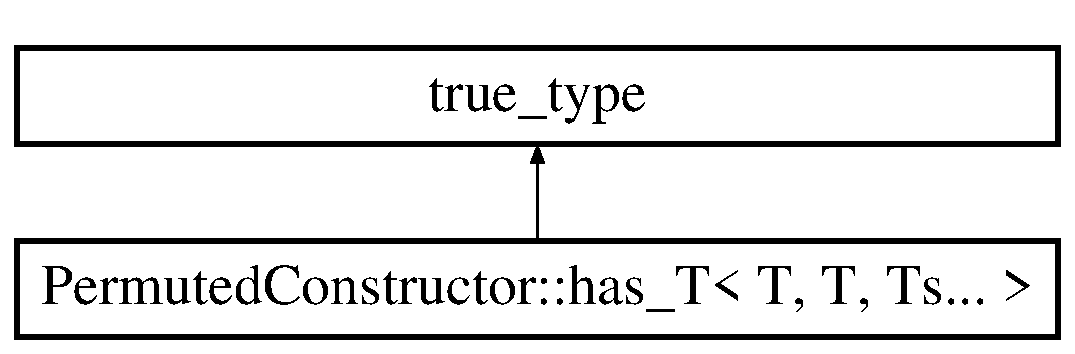
\includegraphics[height=2.000000cm]{struct_permuted_constructor_1_1has___t_3_01_t_00_01_t_00_01_ts_8_8_8_01_4}
\end{center}
\end{figure}


The documentation for this struct was generated from the following file\+:\begin{DoxyCompactItemize}
\item 
Cpp\+Serial\+Port/Serial\+Port.\+h\end{DoxyCompactItemize}

\hypertarget{struct_permuted_constructor_1_1has___t_3_01_t_00_01_tail_00_01_ts_8_8_8_01_4}{}\section{Permuted\+Constructor\+:\+:has\+\_\+T$<$ T, Tail, Ts... $>$ Struct Template Reference}
\label{struct_permuted_constructor_1_1has___t_3_01_t_00_01_tail_00_01_ts_8_8_8_01_4}\index{Permuted\+Constructor\+::has\+\_\+\+T$<$ T, Tail, Ts... $>$@{Permuted\+Constructor\+::has\+\_\+\+T$<$ T, Tail, Ts... $>$}}
Inheritance diagram for Permuted\+Constructor\+:\+:has\+\_\+T$<$ T, Tail, Ts... $>$\+:\begin{figure}[H]
\begin{center}
\leavevmode
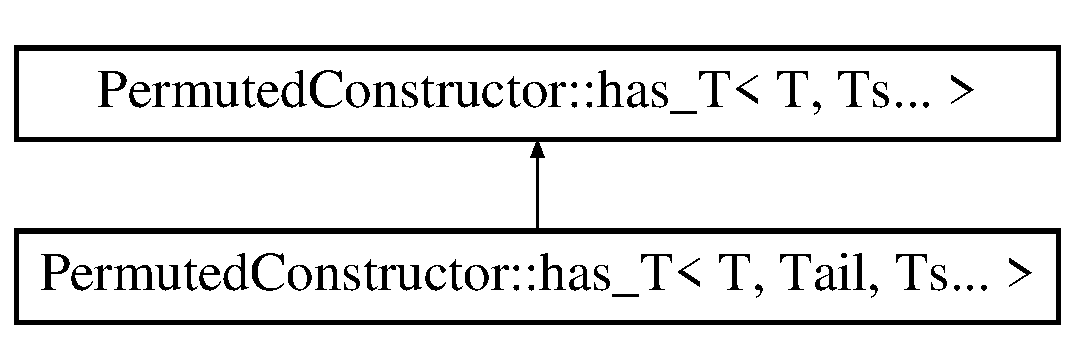
\includegraphics[height=2.000000cm]{struct_permuted_constructor_1_1has___t_3_01_t_00_01_tail_00_01_ts_8_8_8_01_4}
\end{center}
\end{figure}


The documentation for this struct was generated from the following file\+:\begin{DoxyCompactItemize}
\item 
Cpp\+Serial\+Port/Serial\+Port.\+h\end{DoxyCompactItemize}

\hypertarget{class_cpp_serial_port_1_1_i_byte_stream}{}\section{Cpp\+Serial\+Port\+:\+:I\+Byte\+Stream Class Reference}
\label{class_cpp_serial_port_1_1_i_byte_stream}\index{Cpp\+Serial\+Port\+::\+I\+Byte\+Stream@{Cpp\+Serial\+Port\+::\+I\+Byte\+Stream}}
Inheritance diagram for Cpp\+Serial\+Port\+:\+:I\+Byte\+Stream\+:\begin{figure}[H]
\begin{center}
\leavevmode
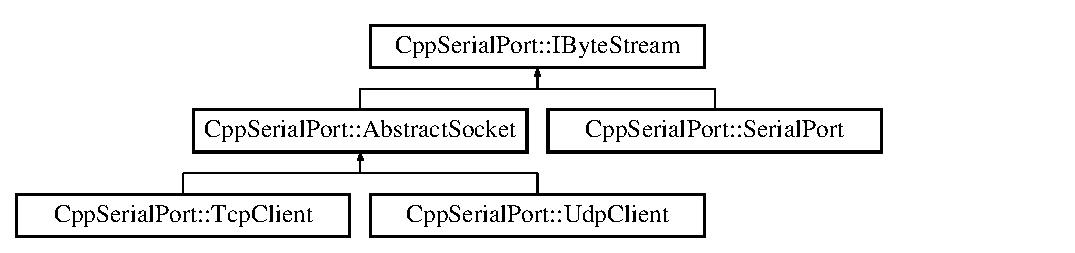
\includegraphics[height=2.947368cm]{class_cpp_serial_port_1_1_i_byte_stream}
\end{center}
\end{figure}
\subsection*{Public Member Functions}
\begin{DoxyCompactItemize}
\item 
\mbox{\Hypertarget{class_cpp_serial_port_1_1_i_byte_stream_af28f2a87feeb1379bc07c0683a701897}\label{class_cpp_serial_port_1_1_i_byte_stream_af28f2a87feeb1379bc07c0683a701897}} 
virtual char {\bfseries read} (bool $\ast$timeout)=0
\item 
\mbox{\Hypertarget{class_cpp_serial_port_1_1_i_byte_stream_af1e8ba6e1cf552c4e5ac0f9b62fa47b1}\label{class_cpp_serial_port_1_1_i_byte_stream_af1e8ba6e1cf552c4e5ac0f9b62fa47b1}} 
virtual ssize\+\_\+t {\bfseries write} (char)=0
\item 
\mbox{\Hypertarget{class_cpp_serial_port_1_1_i_byte_stream_afb3ceb6a2788800baf107e75da33ddd9}\label{class_cpp_serial_port_1_1_i_byte_stream_afb3ceb6a2788800baf107e75da33ddd9}} 
virtual ssize\+\_\+t {\bfseries write} (const char $\ast$, size\+\_\+t)=0
\item 
\mbox{\Hypertarget{class_cpp_serial_port_1_1_i_byte_stream_abb716f1ceedcfbb25c842e95c2838af9}\label{class_cpp_serial_port_1_1_i_byte_stream_abb716f1ceedcfbb25c842e95c2838af9}} 
virtual std\+::string {\bfseries port\+Name} () const =0
\item 
\mbox{\Hypertarget{class_cpp_serial_port_1_1_i_byte_stream_a76ad83842c81e65f90234dc537e08f14}\label{class_cpp_serial_port_1_1_i_byte_stream_a76ad83842c81e65f90234dc537e08f14}} 
virtual bool {\bfseries is\+Open} () const =0
\item 
\mbox{\Hypertarget{class_cpp_serial_port_1_1_i_byte_stream_a4c8932af38cc1e6760c68aba43fa00a1}\label{class_cpp_serial_port_1_1_i_byte_stream_a4c8932af38cc1e6760c68aba43fa00a1}} 
virtual void {\bfseries open\+Port} ()=0
\item 
\mbox{\Hypertarget{class_cpp_serial_port_1_1_i_byte_stream_a630369cad934895644fc809d4bed7490}\label{class_cpp_serial_port_1_1_i_byte_stream_a630369cad934895644fc809d4bed7490}} 
virtual void {\bfseries close\+Port} ()=0
\item 
\mbox{\Hypertarget{class_cpp_serial_port_1_1_i_byte_stream_a8edc9913b52b051abeb187d893b2d50a}\label{class_cpp_serial_port_1_1_i_byte_stream_a8edc9913b52b051abeb187d893b2d50a}} 
virtual void {\bfseries flush\+Rx} ()=0
\item 
\mbox{\Hypertarget{class_cpp_serial_port_1_1_i_byte_stream_af6287327a4b4100c9fb883d117397c3e}\label{class_cpp_serial_port_1_1_i_byte_stream_af6287327a4b4100c9fb883d117397c3e}} 
virtual void {\bfseries flush\+Tx} ()=0
\item 
\mbox{\Hypertarget{class_cpp_serial_port_1_1_i_byte_stream_ab9ea9dadae484027940c5c8af492dad5}\label{class_cpp_serial_port_1_1_i_byte_stream_ab9ea9dadae484027940c5c8af492dad5}} 
virtual size\+\_\+t {\bfseries available} ()=0
\item 
\mbox{\Hypertarget{class_cpp_serial_port_1_1_i_byte_stream_a11f947b7658703eff43ac03af9bf2cc7}\label{class_cpp_serial_port_1_1_i_byte_stream_a11f947b7658703eff43ac03af9bf2cc7}} 
virtual void {\bfseries set\+Read\+Timeout} (int timeout)
\item 
\mbox{\Hypertarget{class_cpp_serial_port_1_1_i_byte_stream_afdfdde0c0622270979106bbb14547580}\label{class_cpp_serial_port_1_1_i_byte_stream_afdfdde0c0622270979106bbb14547580}} 
int {\bfseries read\+Timeout} () const
\item 
\mbox{\Hypertarget{class_cpp_serial_port_1_1_i_byte_stream_a4d141b13df0c151549aacf768581fb4d}\label{class_cpp_serial_port_1_1_i_byte_stream_a4d141b13df0c151549aacf768581fb4d}} 
virtual void {\bfseries set\+Write\+Timeout} (int timeout)
\item 
\mbox{\Hypertarget{class_cpp_serial_port_1_1_i_byte_stream_aeacddd602ce4edb4cccfb6d6eeda1130}\label{class_cpp_serial_port_1_1_i_byte_stream_aeacddd602ce4edb4cccfb6d6eeda1130}} 
int {\bfseries write\+Timeout} () const
\item 
\mbox{\Hypertarget{class_cpp_serial_port_1_1_i_byte_stream_ac03c234ab809736c846931bd275c3dc3}\label{class_cpp_serial_port_1_1_i_byte_stream_ac03c234ab809736c846931bd275c3dc3}} 
\mbox{\hyperlink{class_cpp_serial_port_1_1_byte_array}{Byte\+Array}} {\bfseries line\+Ending} () const
\item 
\mbox{\Hypertarget{class_cpp_serial_port_1_1_i_byte_stream_a33ff07015694cd86a1a03e3ec651580b}\label{class_cpp_serial_port_1_1_i_byte_stream_a33ff07015694cd86a1a03e3ec651580b}} 
void {\bfseries set\+Line\+Ending} (const std\+::string \&str)
\item 
\mbox{\Hypertarget{class_cpp_serial_port_1_1_i_byte_stream_a8766278eb8234c80dda1fb77dbdc3c09}\label{class_cpp_serial_port_1_1_i_byte_stream_a8766278eb8234c80dda1fb77dbdc3c09}} 
void {\bfseries set\+Line\+Ending} (const \mbox{\hyperlink{class_cpp_serial_port_1_1_byte_array}{Byte\+Array}} \&str)
\item 
\mbox{\Hypertarget{class_cpp_serial_port_1_1_i_byte_stream_acf4019b08b1074754bfe4bb575c1d779}\label{class_cpp_serial_port_1_1_i_byte_stream_acf4019b08b1074754bfe4bb575c1d779}} 
void {\bfseries set\+Line\+Ending} (char chr)
\item 
\mbox{\Hypertarget{class_cpp_serial_port_1_1_i_byte_stream_accd239bfab861de9798a7e99bd7a5741}\label{class_cpp_serial_port_1_1_i_byte_stream_accd239bfab861de9798a7e99bd7a5741}} 
virtual ssize\+\_\+t {\bfseries write\+Line} (const std\+::string \&str)
\item 
\mbox{\Hypertarget{class_cpp_serial_port_1_1_i_byte_stream_a620fb9b4891c82f08c896e094f022a78}\label{class_cpp_serial_port_1_1_i_byte_stream_a620fb9b4891c82f08c896e094f022a78}} 
virtual ssize\+\_\+t {\bfseries write\+Line} (const \mbox{\hyperlink{class_cpp_serial_port_1_1_byte_array}{Byte\+Array}} \&byte\+Array)
\item 
\mbox{\Hypertarget{class_cpp_serial_port_1_1_i_byte_stream_a4dbf55370a5ed9f91ac85a387f1f3264}\label{class_cpp_serial_port_1_1_i_byte_stream_a4dbf55370a5ed9f91ac85a387f1f3264}} 
virtual ssize\+\_\+t {\bfseries write} (const \mbox{\hyperlink{class_cpp_serial_port_1_1_byte_array}{Byte\+Array}} \&byte\+Array)
\item 
\mbox{\Hypertarget{class_cpp_serial_port_1_1_i_byte_stream_aab9953fab9e4bccdf09feeaee0a3d93f}\label{class_cpp_serial_port_1_1_i_byte_stream_aab9953fab9e4bccdf09feeaee0a3d93f}} 
virtual \mbox{\hyperlink{class_cpp_serial_port_1_1_byte_array}{Byte\+Array}} {\bfseries read\+Line} (bool $\ast$timeout)
\item 
\mbox{\Hypertarget{class_cpp_serial_port_1_1_i_byte_stream_a6115d8994b068aa1950a68ba84e69941}\label{class_cpp_serial_port_1_1_i_byte_stream_a6115d8994b068aa1950a68ba84e69941}} 
virtual \mbox{\hyperlink{class_cpp_serial_port_1_1_byte_array}{Byte\+Array}} {\bfseries read\+Until} (const \mbox{\hyperlink{class_cpp_serial_port_1_1_byte_array}{Byte\+Array}} \&until, bool $\ast$timeout)
\item 
\mbox{\Hypertarget{class_cpp_serial_port_1_1_i_byte_stream_a7c64aec5e24190acdf210a05b90c7640}\label{class_cpp_serial_port_1_1_i_byte_stream_a7c64aec5e24190acdf210a05b90c7640}} 
virtual \mbox{\hyperlink{class_cpp_serial_port_1_1_byte_array}{Byte\+Array}} {\bfseries read\+Until} (const std\+::string \&until, bool $\ast$timeout)
\item 
\mbox{\Hypertarget{class_cpp_serial_port_1_1_i_byte_stream_a25efa3250fc02ba20151858f4375d02b}\label{class_cpp_serial_port_1_1_i_byte_stream_a25efa3250fc02ba20151858f4375d02b}} 
virtual \mbox{\hyperlink{class_cpp_serial_port_1_1_byte_array}{Byte\+Array}} {\bfseries read\+Until} (char until, bool $\ast$timeout)
\end{DoxyCompactItemize}
\subsection*{Static Protected Member Functions}
\begin{DoxyCompactItemize}
\item 
\mbox{\Hypertarget{class_cpp_serial_port_1_1_i_byte_stream_a47145c37d2b9c4cd5d6c78bb63d398ce}\label{class_cpp_serial_port_1_1_i_byte_stream_a47145c37d2b9c4cd5d6c78bb63d398ce}} 
static bool {\bfseries file\+Exists} (const std\+::string \&file\+Path)
\item 
\mbox{\Hypertarget{class_cpp_serial_port_1_1_i_byte_stream_a36a1dee6f8e03523b8766fd2cda5569e}\label{class_cpp_serial_port_1_1_i_byte_stream_a36a1dee6f8e03523b8766fd2cda5569e}} 
{\footnotesize template$<$typename T $>$ }\\static std\+::string {\bfseries to\+Std\+String} (const T \&t)
\item 
\mbox{\Hypertarget{class_cpp_serial_port_1_1_i_byte_stream_a037ef7054280feff00160b0a7818e897}\label{class_cpp_serial_port_1_1_i_byte_stream_a037ef7054280feff00160b0a7818e897}} 
static std\+::string {\bfseries strip\+Line\+Endings} (const std\+::string \&input)
\item 
\mbox{\Hypertarget{class_cpp_serial_port_1_1_i_byte_stream_ab9b56a8ae6ee5e3d1bf100d91b0adc18}\label{class_cpp_serial_port_1_1_i_byte_stream_ab9b56a8ae6ee5e3d1bf100d91b0adc18}} 
static uint64\+\_\+t {\bfseries get\+Epoch} ()
\end{DoxyCompactItemize}
\subsection*{Static Protected Attributes}
\begin{DoxyCompactItemize}
\item 
\mbox{\Hypertarget{class_cpp_serial_port_1_1_i_byte_stream_ae896f7775f1926653bb001f15c770b30}\label{class_cpp_serial_port_1_1_i_byte_stream_ae896f7775f1926653bb001f15c770b30}} 
static const int {\bfseries D\+E\+F\+A\+U\+L\+T\+\_\+\+R\+E\+A\+D\+\_\+\+T\+I\+M\+E\+O\+UT} \{1000\}
\item 
\mbox{\Hypertarget{class_cpp_serial_port_1_1_i_byte_stream_a3d0ef76dc1ba015626384d3801b51b08}\label{class_cpp_serial_port_1_1_i_byte_stream_a3d0ef76dc1ba015626384d3801b51b08}} 
static const int {\bfseries D\+E\+F\+A\+U\+L\+T\+\_\+\+W\+R\+I\+T\+E\+\_\+\+T\+I\+M\+E\+O\+UT} \{1000\}
\end{DoxyCompactItemize}


The documentation for this class was generated from the following files\+:\begin{DoxyCompactItemize}
\item 
Cpp\+Serial\+Port/I\+Byte\+Stream.\+h\item 
Cpp\+Serial\+Port/I\+Byte\+Stream.\+cpp\end{DoxyCompactItemize}

\hypertarget{class_cpp_serial_port_1_1_i_p_v4_address}{}\section{Cpp\+Serial\+Port\+:\+:I\+P\+V4\+Address Class Reference}
\label{class_cpp_serial_port_1_1_i_p_v4_address}\index{Cpp\+Serial\+Port\+::\+I\+P\+V4\+Address@{Cpp\+Serial\+Port\+::\+I\+P\+V4\+Address}}
\subsection*{Public Member Functions}
\begin{DoxyCompactItemize}
\item 
\mbox{\Hypertarget{class_cpp_serial_port_1_1_i_p_v4_address_aca670bf2187bad7617f611dc0e1f111f}\label{class_cpp_serial_port_1_1_i_p_v4_address_aca670bf2187bad7617f611dc0e1f111f}} 
{\bfseries I\+P\+V4\+Address} (uint32\+\_\+t address)
\item 
\mbox{\Hypertarget{class_cpp_serial_port_1_1_i_p_v4_address_afaf6fc9748451e32cfd6414f38af98c2}\label{class_cpp_serial_port_1_1_i_p_v4_address_afaf6fc9748451e32cfd6414f38af98c2}} 
{\bfseries I\+P\+V4\+Address} (uint8\+\_\+t $\ast$bytes)
\item 
\mbox{\Hypertarget{class_cpp_serial_port_1_1_i_p_v4_address_a44f1afc69207730a48e181bf61a40f40}\label{class_cpp_serial_port_1_1_i_p_v4_address_a44f1afc69207730a48e181bf61a40f40}} 
{\bfseries I\+P\+V4\+Address} (const uint8\+\_\+t $\ast$bytes)
\item 
\mbox{\Hypertarget{class_cpp_serial_port_1_1_i_p_v4_address_a0d2c74afaa60975d339ebece26cae883}\label{class_cpp_serial_port_1_1_i_p_v4_address_a0d2c74afaa60975d339ebece26cae883}} 
{\bfseries I\+P\+V4\+Address} (uint8\+\_\+t byte0, uint8\+\_\+t byte1, uint8\+\_\+t byte2, uint8\+\_\+t byte3)
\item 
\mbox{\Hypertarget{class_cpp_serial_port_1_1_i_p_v4_address_a1680c018e692048fb7a5e54c742ad72e}\label{class_cpp_serial_port_1_1_i_p_v4_address_a1680c018e692048fb7a5e54c742ad72e}} 
uint8\+\_\+t \& {\bfseries operator\mbox{[}$\,$\mbox{]}} (size\+\_\+t index)
\item 
\mbox{\Hypertarget{class_cpp_serial_port_1_1_i_p_v4_address_a598b9c9faa71ab44e6d99454f92ab048}\label{class_cpp_serial_port_1_1_i_p_v4_address_a598b9c9faa71ab44e6d99454f92ab048}} 
const uint8\+\_\+t \& {\bfseries operator\mbox{[}$\,$\mbox{]}} (size\+\_\+t index) const
\item 
\mbox{\Hypertarget{class_cpp_serial_port_1_1_i_p_v4_address_ab326d8fd9b00adc5066e8087334c49d1}\label{class_cpp_serial_port_1_1_i_p_v4_address_ab326d8fd9b00adc5066e8087334c49d1}} 
uint32\+\_\+t \& {\bfseries address} ()
\item 
\mbox{\Hypertarget{class_cpp_serial_port_1_1_i_p_v4_address_a5d25fb1563ac1a681e29609dd32f80ea}\label{class_cpp_serial_port_1_1_i_p_v4_address_a5d25fb1563ac1a681e29609dd32f80ea}} 
const uint32\+\_\+t \& {\bfseries address} () const
\item 
\mbox{\Hypertarget{class_cpp_serial_port_1_1_i_p_v4_address_a28de245ff940b05d2bb11f550d5ed5ab}\label{class_cpp_serial_port_1_1_i_p_v4_address_a28de245ff940b05d2bb11f550d5ed5ab}} 
std\+::string {\bfseries to\+String} () const
\end{DoxyCompactItemize}


The documentation for this class was generated from the following files\+:\begin{DoxyCompactItemize}
\item 
Cpp\+Serial\+Port/I\+P\+V4\+Address.\+h\item 
Cpp\+Serial\+Port/I\+P\+V4\+Address.\+cpp\end{DoxyCompactItemize}

\hypertarget{struct_permuted_constructor_1_1is__included}{}\section{Permuted\+Constructor\+:\+:is\+\_\+included$<$ T1, T2 $>$ Struct Template Reference}
\label{struct_permuted_constructor_1_1is__included}\index{Permuted\+Constructor\+::is\+\_\+included$<$ T1, T2 $>$@{Permuted\+Constructor\+::is\+\_\+included$<$ T1, T2 $>$}}


The documentation for this struct was generated from the following file\+:\begin{DoxyCompactItemize}
\item 
Cpp\+Serial\+Port/Serial\+Port.\+h\end{DoxyCompactItemize}

\hypertarget{struct_permuted_constructor_1_1is__included_3_01std_1_1tuple_3_01_t_00_01_ts_8_8_8_01_4_00_01std7773b1cf7a852a22f74d472d1ee753c4}{}\section{Permuted\+Constructor\+:\+:is\+\_\+included$<$ std\+:\+:tuple$<$ T, Ts... $>$, std\+:\+:tuple$<$ Ts2... $>$ $>$ Struct Template Reference}
\label{struct_permuted_constructor_1_1is__included_3_01std_1_1tuple_3_01_t_00_01_ts_8_8_8_01_4_00_01std7773b1cf7a852a22f74d472d1ee753c4}\index{Permuted\+Constructor\+::is\+\_\+included$<$ std\+::tuple$<$ T, Ts... $>$, std\+::tuple$<$ Ts2... $>$ $>$@{Permuted\+Constructor\+::is\+\_\+included$<$ std\+::tuple$<$ T, Ts... $>$, std\+::tuple$<$ Ts2... $>$ $>$}}
Inheritance diagram for Permuted\+Constructor\+:\+:is\+\_\+included$<$ std\+:\+:tuple$<$ T, Ts... $>$, std\+:\+:tuple$<$ Ts2... $>$ $>$\+:\begin{figure}[H]
\begin{center}
\leavevmode
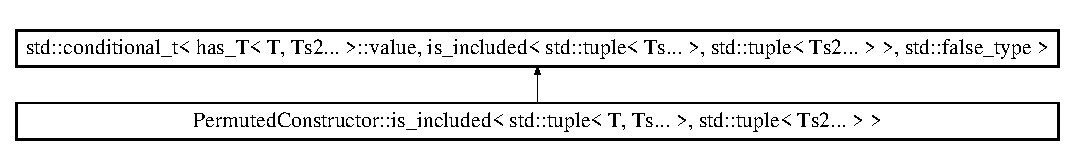
\includegraphics[height=1.651917cm]{struct_permuted_constructor_1_1is__included_3_01std_1_1tuple_3_01_t_00_01_ts_8_8_8_01_4_00_01std7773b1cf7a852a22f74d472d1ee753c4}
\end{center}
\end{figure}


The documentation for this struct was generated from the following file\+:\begin{DoxyCompactItemize}
\item 
Cpp\+Serial\+Port/Serial\+Port.\+h\end{DoxyCompactItemize}

\hypertarget{struct_permuted_constructor_1_1is__included_3_01std_1_1tuple_3_4_00_01std_1_1tuple_3_01_ts_8_8_8_01_4_01_4}{}\section{Permuted\+Constructor\+:\+:is\+\_\+included$<$ std\+:\+:tuple$<$$>$, std\+:\+:tuple$<$ Ts... $>$ $>$ Struct Template Reference}
\label{struct_permuted_constructor_1_1is__included_3_01std_1_1tuple_3_4_00_01std_1_1tuple_3_01_ts_8_8_8_01_4_01_4}\index{Permuted\+Constructor\+::is\+\_\+included$<$ std\+::tuple$<$$>$, std\+::tuple$<$ Ts... $>$ $>$@{Permuted\+Constructor\+::is\+\_\+included$<$ std\+::tuple$<$$>$, std\+::tuple$<$ Ts... $>$ $>$}}
Inheritance diagram for Permuted\+Constructor\+:\+:is\+\_\+included$<$ std\+:\+:tuple$<$$>$, std\+:\+:tuple$<$ Ts... $>$ $>$\+:\begin{figure}[H]
\begin{center}
\leavevmode
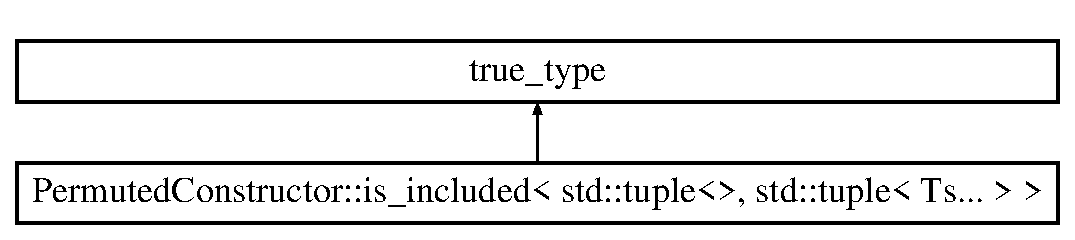
\includegraphics[height=2.000000cm]{struct_permuted_constructor_1_1is__included_3_01std_1_1tuple_3_4_00_01std_1_1tuple_3_01_ts_8_8_8_01_4_01_4}
\end{center}
\end{figure}


The documentation for this struct was generated from the following file\+:\begin{DoxyCompactItemize}
\item 
Cpp\+Serial\+Port/Serial\+Port.\+h\end{DoxyCompactItemize}

\hypertarget{class_cpp_serial_port_1_1_serial_port}{}\section{Cpp\+Serial\+Port\+:\+:Serial\+Port Class Reference}
\label{class_cpp_serial_port_1_1_serial_port}\index{Cpp\+Serial\+Port\+::\+Serial\+Port@{Cpp\+Serial\+Port\+::\+Serial\+Port}}
Inheritance diagram for Cpp\+Serial\+Port\+:\+:Serial\+Port\+:\begin{figure}[H]
\begin{center}
\leavevmode
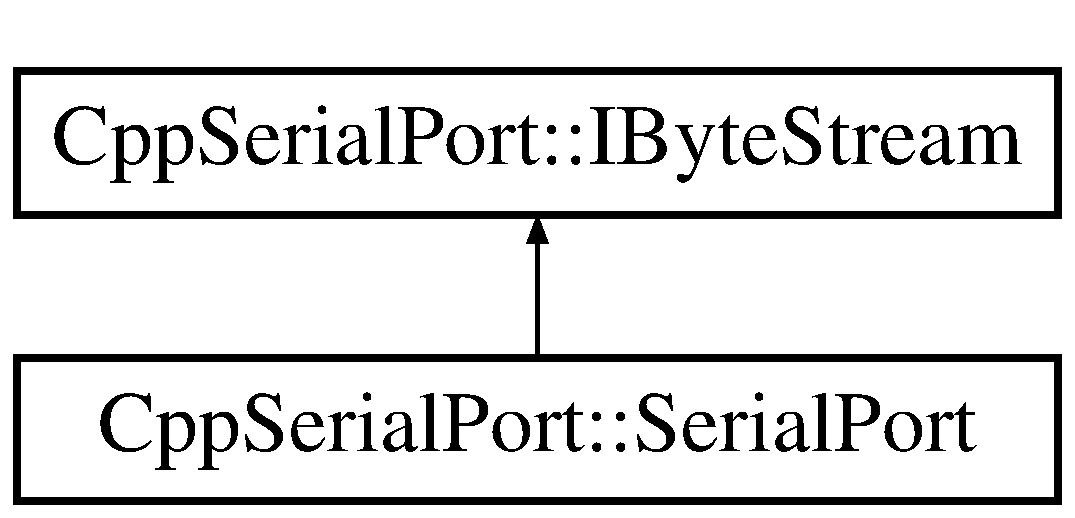
\includegraphics[height=2.000000cm]{class_cpp_serial_port_1_1_serial_port}
\end{center}
\end{figure}
\subsection*{Public Member Functions}
\begin{DoxyCompactItemize}
\item 
\mbox{\Hypertarget{class_cpp_serial_port_1_1_serial_port_a42360a1556f13c1dd73f31d5e1210194}\label{class_cpp_serial_port_1_1_serial_port_a42360a1556f13c1dd73f31d5e1210194}} 
{\bfseries Serial\+Port} (const std\+::string \&name, Baud\+Rate baud\+Rate=D\+E\+F\+A\+U\+L\+T\+\_\+\+B\+A\+U\+D\+\_\+\+R\+A\+TE, Data\+Bits data\+Bits=D\+E\+F\+A\+U\+L\+T\+\_\+\+D\+A\+T\+A\+\_\+\+B\+I\+TS, Stop\+Bits stop\+Bits=D\+E\+F\+A\+U\+L\+T\+\_\+\+S\+T\+O\+P\+\_\+\+B\+I\+TS, Parity parity=D\+E\+F\+A\+U\+L\+T\+\_\+\+P\+A\+R\+I\+TY, Flow\+Control flow\+Control=D\+E\+F\+A\+U\+L\+T\+\_\+\+F\+L\+O\+W\+\_\+\+C\+O\+N\+T\+R\+OL, const std\+::string \&line\+Ending=D\+E\+F\+A\+U\+L\+T\+\_\+\+L\+I\+N\+E\+\_\+\+E\+N\+D\+I\+NG)
\item 
\mbox{\Hypertarget{class_cpp_serial_port_1_1_serial_port_af4d689fc5fe9bcab53d1d373cbaeabb1}\label{class_cpp_serial_port_1_1_serial_port_af4d689fc5fe9bcab53d1d373cbaeabb1}} 
{\footnotesize template$<$typename ... Ts, typename std\+::enable\+\_\+if\+\_\+t$<$ Permuted\+Constructor\+::is\+\_\+included$<$ std\+::tuple$<$ Ts... $>$, std\+::tuple$<$ const std\+::string \&, Baud\+Rate, Data\+Bits, Stop\+Bits, Parity, Flow\+Control, const std\+::string \&$>$$>$\+::value $>$ $\ast$  = nullptr$>$ }\\{\bfseries Serial\+Port} (const Ts \&... ts)
\item 
\mbox{\Hypertarget{class_cpp_serial_port_1_1_serial_port_af7a749032a61ed92de0654d076e7e46c}\label{class_cpp_serial_port_1_1_serial_port_af7a749032a61ed92de0654d076e7e46c}} 
{\bfseries Serial\+Port} (\mbox{\hyperlink{class_cpp_serial_port_1_1_serial_port}{Serial\+Port}} \&\&other)=delete
\item 
\mbox{\Hypertarget{class_cpp_serial_port_1_1_serial_port_ad9f57729bd109a8630f495b6d63bc8a7}\label{class_cpp_serial_port_1_1_serial_port_ad9f57729bd109a8630f495b6d63bc8a7}} 
\mbox{\hyperlink{class_cpp_serial_port_1_1_serial_port}{Serial\+Port}} \& {\bfseries operator=} (const \mbox{\hyperlink{class_cpp_serial_port_1_1_serial_port}{Serial\+Port}} \&rhs)=delete
\item 
\mbox{\Hypertarget{class_cpp_serial_port_1_1_serial_port_a220dd4de1d53f2f5a11201f0220ec578}\label{class_cpp_serial_port_1_1_serial_port_a220dd4de1d53f2f5a11201f0220ec578}} 
\mbox{\hyperlink{class_cpp_serial_port_1_1_serial_port}{Serial\+Port}} \& {\bfseries operator=} (\mbox{\hyperlink{class_cpp_serial_port_1_1_serial_port}{Serial\+Port}} \&\&rhs)=delete
\item 
\mbox{\Hypertarget{class_cpp_serial_port_1_1_serial_port_aeee886c2522295c54b03c815d5d2de34}\label{class_cpp_serial_port_1_1_serial_port_aeee886c2522295c54b03c815d5d2de34}} 
{\bfseries Serial\+Port} (const \mbox{\hyperlink{class_cpp_serial_port_1_1_serial_port}{Serial\+Port}} \&other)=delete
\item 
\mbox{\Hypertarget{class_cpp_serial_port_1_1_serial_port_a0f2a02548c03ceaf52e2591d6641fd53}\label{class_cpp_serial_port_1_1_serial_port_a0f2a02548c03ceaf52e2591d6641fd53}} 
void \mbox{\hyperlink{class_cpp_serial_port_1_1_serial_port_a0f2a02548c03ceaf52e2591d6641fd53}{open\+Port}} () override
\begin{DoxyCompactList}\small\item\em defined(\+\_\+\+W\+I\+N32) \end{DoxyCompactList}\item 
\mbox{\Hypertarget{class_cpp_serial_port_1_1_serial_port_a88d33aefcab3675a673f7a747d9cc662}\label{class_cpp_serial_port_1_1_serial_port_a88d33aefcab3675a673f7a747d9cc662}} 
void {\bfseries close\+Port} () override
\item 
\mbox{\Hypertarget{class_cpp_serial_port_1_1_serial_port_a371a76a8dba93882f2c23d3aaf2a08d1}\label{class_cpp_serial_port_1_1_serial_port_a371a76a8dba93882f2c23d3aaf2a08d1}} 
char {\bfseries read} (bool $\ast$read\+Timeout) override
\item 
\mbox{\Hypertarget{class_cpp_serial_port_1_1_serial_port_a0fe57db7f9f76f280b0bb3e71eb85e82}\label{class_cpp_serial_port_1_1_serial_port_a0fe57db7f9f76f280b0bb3e71eb85e82}} 
void {\bfseries set\+Read\+Timeout} (int timeout) override
\item 
\mbox{\Hypertarget{class_cpp_serial_port_1_1_serial_port_a19b64e0ad5cc85abc6986d95b294270b}\label{class_cpp_serial_port_1_1_serial_port_a19b64e0ad5cc85abc6986d95b294270b}} 
std\+::string {\bfseries port\+Name} () const override
\item 
\mbox{\Hypertarget{class_cpp_serial_port_1_1_serial_port_a042486989f96cfd7add00b827dca45b4}\label{class_cpp_serial_port_1_1_serial_port_a042486989f96cfd7add00b827dca45b4}} 
bool {\bfseries is\+Open} () const override
\item 
\mbox{\Hypertarget{class_cpp_serial_port_1_1_serial_port_aaf74f8d3d23a92168e5833505f840f04}\label{class_cpp_serial_port_1_1_serial_port_aaf74f8d3d23a92168e5833505f840f04}} 
bool {\bfseries is\+D\+C\+D\+Enabled} () const
\item 
\mbox{\Hypertarget{class_cpp_serial_port_1_1_serial_port_a64c3fbb406cd712e7044ba06d7a12dec}\label{class_cpp_serial_port_1_1_serial_port_a64c3fbb406cd712e7044ba06d7a12dec}} 
bool {\bfseries is\+C\+T\+S\+Enabled} () const
\item 
\mbox{\Hypertarget{class_cpp_serial_port_1_1_serial_port_a698511a12a1b5d81294fe93d39a00b24}\label{class_cpp_serial_port_1_1_serial_port_a698511a12a1b5d81294fe93d39a00b24}} 
bool {\bfseries is\+D\+S\+R\+Enabled} () const
\item 
\mbox{\Hypertarget{class_cpp_serial_port_1_1_serial_port_afd1986e6e55778e8cec73aff6bba3af8}\label{class_cpp_serial_port_1_1_serial_port_afd1986e6e55778e8cec73aff6bba3af8}} 
void {\bfseries enable\+D\+TR} ()
\item 
\mbox{\Hypertarget{class_cpp_serial_port_1_1_serial_port_ab2a039d398a524044684f11f13b9172e}\label{class_cpp_serial_port_1_1_serial_port_ab2a039d398a524044684f11f13b9172e}} 
void {\bfseries disable\+D\+TR} ()
\item 
\mbox{\Hypertarget{class_cpp_serial_port_1_1_serial_port_a0f3256bbedfef4bdc7b0ad7bd2da4ca9}\label{class_cpp_serial_port_1_1_serial_port_a0f3256bbedfef4bdc7b0ad7bd2da4ca9}} 
void {\bfseries enable\+R\+TS} ()
\item 
\mbox{\Hypertarget{class_cpp_serial_port_1_1_serial_port_a0bf70c7ca280941b1b1b2f834c47ea27}\label{class_cpp_serial_port_1_1_serial_port_a0bf70c7ca280941b1b1b2f834c47ea27}} 
void {\bfseries disable\+R\+TS} ()
\item 
\mbox{\Hypertarget{class_cpp_serial_port_1_1_serial_port_a4951d7dcfe2b8a53f6a49f71f971f81a}\label{class_cpp_serial_port_1_1_serial_port_a4951d7dcfe2b8a53f6a49f71f971f81a}} 
void {\bfseries flush\+Rx} () override
\item 
\mbox{\Hypertarget{class_cpp_serial_port_1_1_serial_port_a6731e2f4285f36f0af1cc494108ffe17}\label{class_cpp_serial_port_1_1_serial_port_a6731e2f4285f36f0af1cc494108ffe17}} 
void {\bfseries flush\+Tx} () override
\item 
\mbox{\Hypertarget{class_cpp_serial_port_1_1_serial_port_a5c44fe416c7c97aaf31d4d9264eee24a}\label{class_cpp_serial_port_1_1_serial_port_a5c44fe416c7c97aaf31d4d9264eee24a}} 
ssize\+\_\+t {\bfseries write} (char c) override
\item 
\mbox{\Hypertarget{class_cpp_serial_port_1_1_serial_port_ae8a9bf74cc699adac92cd710c3179b97}\label{class_cpp_serial_port_1_1_serial_port_ae8a9bf74cc699adac92cd710c3179b97}} 
ssize\+\_\+t {\bfseries write} (const char $\ast$bytes, size\+\_\+t number\+Of\+Bytes) override
\item 
\mbox{\Hypertarget{class_cpp_serial_port_1_1_serial_port_a1d7dcc29d1119cd653702056522e5896}\label{class_cpp_serial_port_1_1_serial_port_a1d7dcc29d1119cd653702056522e5896}} 
size\+\_\+t {\bfseries available} () override
\item 
\mbox{\Hypertarget{class_cpp_serial_port_1_1_serial_port_a476ac7cf164b4e5032e678e40fe55fed}\label{class_cpp_serial_port_1_1_serial_port_a476ac7cf164b4e5032e678e40fe55fed}} 
void {\bfseries set\+Baud\+Rate} (Baud\+Rate baud\+Rate)
\item 
\mbox{\Hypertarget{class_cpp_serial_port_1_1_serial_port_a85e821679d098c7a245ddefd7afe8794}\label{class_cpp_serial_port_1_1_serial_port_a85e821679d098c7a245ddefd7afe8794}} 
void {\bfseries set\+Stop\+Bits} (Stop\+Bits stop\+Bits)
\item 
\mbox{\Hypertarget{class_cpp_serial_port_1_1_serial_port_acd40e1ddd34b2355aa1f44a199b76ee1}\label{class_cpp_serial_port_1_1_serial_port_acd40e1ddd34b2355aa1f44a199b76ee1}} 
void {\bfseries set\+Parity} (Parity parity)
\item 
\mbox{\Hypertarget{class_cpp_serial_port_1_1_serial_port_af827625d50ff19658cd1ef4cd6ceadf4}\label{class_cpp_serial_port_1_1_serial_port_af827625d50ff19658cd1ef4cd6ceadf4}} 
void {\bfseries set\+Data\+Bits} (Data\+Bits data\+Bits)
\item 
\mbox{\Hypertarget{class_cpp_serial_port_1_1_serial_port_afc245ca341189ccce0635a23d55ca62d}\label{class_cpp_serial_port_1_1_serial_port_afc245ca341189ccce0635a23d55ca62d}} 
void {\bfseries set\+Flow\+Control} (Flow\+Control flow\+Control)
\item 
\mbox{\Hypertarget{class_cpp_serial_port_1_1_serial_port_abd4697780fd17ce3e6db0f7b8fb8aaab}\label{class_cpp_serial_port_1_1_serial_port_abd4697780fd17ce3e6db0f7b8fb8aaab}} 
Baud\+Rate {\bfseries baud\+Rate} () const
\item 
\mbox{\Hypertarget{class_cpp_serial_port_1_1_serial_port_aa8d6f6636e1d2979c63f31a537cc8d74}\label{class_cpp_serial_port_1_1_serial_port_aa8d6f6636e1d2979c63f31a537cc8d74}} 
Stop\+Bits {\bfseries stop\+Bits} () const
\item 
\mbox{\Hypertarget{class_cpp_serial_port_1_1_serial_port_ac43fb422fb778e9a6f79af1ab8e060db}\label{class_cpp_serial_port_1_1_serial_port_ac43fb422fb778e9a6f79af1ab8e060db}} 
Data\+Bits {\bfseries data\+Bits} () const
\item 
\mbox{\Hypertarget{class_cpp_serial_port_1_1_serial_port_ab2dbea9d01bc345b835b3552c29acace}\label{class_cpp_serial_port_1_1_serial_port_ab2dbea9d01bc345b835b3552c29acace}} 
Parity {\bfseries parity} () const
\item 
\mbox{\Hypertarget{class_cpp_serial_port_1_1_serial_port_a5ccf8c9d17e3ac4697b2ff01082e718d}\label{class_cpp_serial_port_1_1_serial_port_a5ccf8c9d17e3ac4697b2ff01082e718d}} 
Flow\+Control {\bfseries flow\+Control} () const
\end{DoxyCompactItemize}
\subsection*{Static Public Member Functions}
\begin{DoxyCompactItemize}
\item 
\mbox{\Hypertarget{class_cpp_serial_port_1_1_serial_port_a0f7b939f57e91bd7f9ca8bce0b90a118}\label{class_cpp_serial_port_1_1_serial_port_a0f7b939f57e91bd7f9ca8bce0b90a118}} 
static std\+::unordered\+\_\+set$<$ std\+::string $>$ {\bfseries available\+Serial\+Ports} ()
\item 
\mbox{\Hypertarget{class_cpp_serial_port_1_1_serial_port_aacc6ad3a34fe8b998858db42353ba8e5}\label{class_cpp_serial_port_1_1_serial_port_aacc6ad3a34fe8b998858db42353ba8e5}} 
static bool {\bfseries is\+Valid\+Serial\+Port\+Name} (const std\+::string \&serial\+Port\+Name)
\item 
\mbox{\Hypertarget{class_cpp_serial_port_1_1_serial_port_a7410880357c66fa7d742a66865c85055}\label{class_cpp_serial_port_1_1_serial_port_a7410880357c66fa7d742a66865c85055}} 
static bool {\bfseries is\+Available\+Serial\+Port} (const std\+::string \&name)
\end{DoxyCompactItemize}
\subsection*{Static Public Attributes}
\begin{DoxyCompactItemize}
\item 
\mbox{\Hypertarget{class_cpp_serial_port_1_1_serial_port_a654c959db8c2aec6ae8c2101bc28c74e}\label{class_cpp_serial_port_1_1_serial_port_a654c959db8c2aec6ae8c2101bc28c74e}} 
static const Stop\+Bits {\bfseries D\+E\+F\+A\+U\+L\+T\+\_\+\+S\+T\+O\+P\+\_\+\+B\+I\+TS} \{Stop\+Bits\+::\+Stop\+One\}
\item 
\mbox{\Hypertarget{class_cpp_serial_port_1_1_serial_port_a9d6e1bfb16a9281cb3bde9d74118a022}\label{class_cpp_serial_port_1_1_serial_port_a9d6e1bfb16a9281cb3bde9d74118a022}} 
static const Parity {\bfseries D\+E\+F\+A\+U\+L\+T\+\_\+\+P\+A\+R\+I\+TY} \{Parity\+::\+Parity\+None\}
\item 
\mbox{\Hypertarget{class_cpp_serial_port_1_1_serial_port_a2140def05b9ef513defcd558a6f76bf5}\label{class_cpp_serial_port_1_1_serial_port_a2140def05b9ef513defcd558a6f76bf5}} 
static const Baud\+Rate {\bfseries D\+E\+F\+A\+U\+L\+T\+\_\+\+B\+A\+U\+D\+\_\+\+R\+A\+TE} \{Baud\+Rate\+::\+Baud9600\}
\item 
\mbox{\Hypertarget{class_cpp_serial_port_1_1_serial_port_a7580640725498c24a02c0683cda290d4}\label{class_cpp_serial_port_1_1_serial_port_a7580640725498c24a02c0683cda290d4}} 
static const Data\+Bits {\bfseries D\+E\+F\+A\+U\+L\+T\+\_\+\+D\+A\+T\+A\+\_\+\+B\+I\+TS} \{Data\+Bits\+::\+Data\+Eight\}
\item 
\mbox{\Hypertarget{class_cpp_serial_port_1_1_serial_port_ac4b188c8e479c7b555f3375243ffce88}\label{class_cpp_serial_port_1_1_serial_port_ac4b188c8e479c7b555f3375243ffce88}} 
static const Flow\+Control {\bfseries D\+E\+F\+A\+U\+L\+T\+\_\+\+F\+L\+O\+W\+\_\+\+C\+O\+N\+T\+R\+OL} \{Flow\+Control\+::\+Flow\+Off\}
\item 
\mbox{\Hypertarget{class_cpp_serial_port_1_1_serial_port_a2f7f96304dbc01de3b3d1526a692ca90}\label{class_cpp_serial_port_1_1_serial_port_a2f7f96304dbc01de3b3d1526a692ca90}} 
static const std\+::string {\bfseries D\+E\+F\+A\+U\+L\+T\+\_\+\+L\+I\+N\+E\+\_\+\+E\+N\+D\+I\+NG} \{\char`\"{}\textbackslash{}n\char`\"{}\}
\item 
\mbox{\Hypertarget{class_cpp_serial_port_1_1_serial_port_aeef5352ca5292a399e0d36f5af74a23b}\label{class_cpp_serial_port_1_1_serial_port_aeef5352ca5292a399e0d36f5af74a23b}} 
static const long {\bfseries D\+E\+F\+A\+U\+L\+T\+\_\+\+R\+E\+T\+R\+Y\+\_\+\+C\+O\+U\+NT}
\end{DoxyCompactItemize}
\subsection*{Additional Inherited Members}


The documentation for this class was generated from the following files\+:\begin{DoxyCompactItemize}
\item 
Cpp\+Serial\+Port/Serial\+Port.\+h\item 
Cpp\+Serial\+Port/Serial\+Port.\+cpp\end{DoxyCompactItemize}

\hypertarget{class_cpp_serial_port_1_1_serial_port_disconnected_exception}{}\section{Cpp\+Serial\+Port\+:\+:Serial\+Port\+Disconnected\+Exception Class Reference}
\label{class_cpp_serial_port_1_1_serial_port_disconnected_exception}\index{Cpp\+Serial\+Port\+::\+Serial\+Port\+Disconnected\+Exception@{Cpp\+Serial\+Port\+::\+Serial\+Port\+Disconnected\+Exception}}
Inheritance diagram for Cpp\+Serial\+Port\+:\+:Serial\+Port\+Disconnected\+Exception\+:\begin{figure}[H]
\begin{center}
\leavevmode
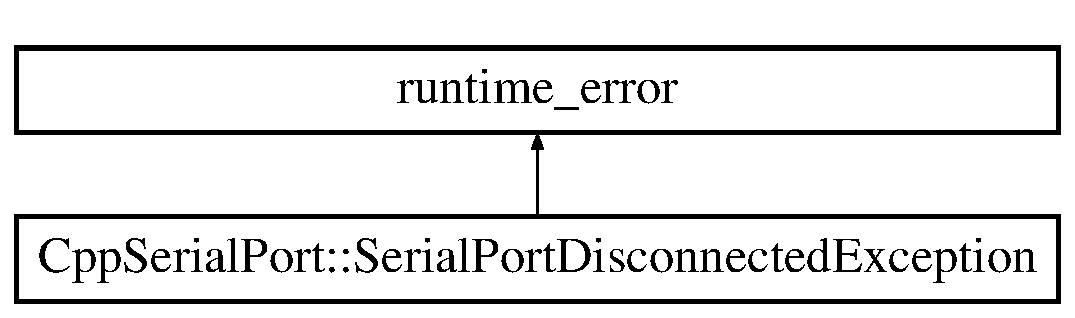
\includegraphics[height=2.000000cm]{class_cpp_serial_port_1_1_serial_port_disconnected_exception}
\end{center}
\end{figure}
\subsection*{Public Member Functions}
\begin{DoxyCompactItemize}
\item 
\mbox{\Hypertarget{class_cpp_serial_port_1_1_serial_port_disconnected_exception_afb00f2aba1cc7aa2bf956a88a6885fde}\label{class_cpp_serial_port_1_1_serial_port_disconnected_exception_afb00f2aba1cc7aa2bf956a88a6885fde}} 
{\bfseries Serial\+Port\+Disconnected\+Exception} (const std\+::string \&port\+Name, const std\+::string \&what)
\item 
\mbox{\Hypertarget{class_cpp_serial_port_1_1_serial_port_disconnected_exception_ad2026ae9ebb13be071eaad93a86f125a}\label{class_cpp_serial_port_1_1_serial_port_disconnected_exception_ad2026ae9ebb13be071eaad93a86f125a}} 
std\+::string {\bfseries port\+Name} () const
\item 
\mbox{\Hypertarget{class_cpp_serial_port_1_1_serial_port_disconnected_exception_a1514d0c574d676b9625a988dc5ee64c5}\label{class_cpp_serial_port_1_1_serial_port_disconnected_exception_a1514d0c574d676b9625a988dc5ee64c5}} 
void {\bfseries set\+Port\+Name} (const std\+::string \&port\+Name)
\end{DoxyCompactItemize}


The documentation for this class was generated from the following file\+:\begin{DoxyCompactItemize}
\item 
Cpp\+Serial\+Port/Serial\+Port.\+h\end{DoxyCompactItemize}

\hypertarget{class_cpp_serial_port_1_1_socket_disconnected_exception}{}\section{Cpp\+Serial\+Port\+:\+:Socket\+Disconnected\+Exception Class Reference}
\label{class_cpp_serial_port_1_1_socket_disconnected_exception}\index{Cpp\+Serial\+Port\+::\+Socket\+Disconnected\+Exception@{Cpp\+Serial\+Port\+::\+Socket\+Disconnected\+Exception}}
Inheritance diagram for Cpp\+Serial\+Port\+:\+:Socket\+Disconnected\+Exception\+:\begin{figure}[H]
\begin{center}
\leavevmode
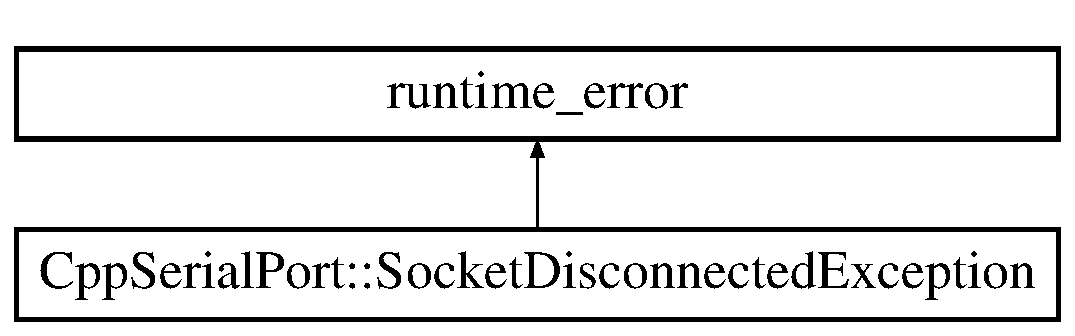
\includegraphics[height=2.000000cm]{class_cpp_serial_port_1_1_socket_disconnected_exception}
\end{center}
\end{figure}
\subsection*{Public Member Functions}
\begin{DoxyCompactItemize}
\item 
\mbox{\Hypertarget{class_cpp_serial_port_1_1_socket_disconnected_exception_a720ff500086197ae055279f76715254e}\label{class_cpp_serial_port_1_1_socket_disconnected_exception_a720ff500086197ae055279f76715254e}} 
{\bfseries Socket\+Disconnected\+Exception} (const std\+::string \&port\+Name, const std\+::string \&what)
\item 
\mbox{\Hypertarget{class_cpp_serial_port_1_1_socket_disconnected_exception_aa427a8398db0b5bb33ef5fbbdf83503a}\label{class_cpp_serial_port_1_1_socket_disconnected_exception_aa427a8398db0b5bb33ef5fbbdf83503a}} 
std\+::string {\bfseries port\+Name} () const
\item 
\mbox{\Hypertarget{class_cpp_serial_port_1_1_socket_disconnected_exception_a8734a849717a23db8ce672ce6b0196c6}\label{class_cpp_serial_port_1_1_socket_disconnected_exception_a8734a849717a23db8ce672ce6b0196c6}} 
void {\bfseries set\+Port\+Name} (const std\+::string \&port\+Name)
\end{DoxyCompactItemize}


The documentation for this class was generated from the following file\+:\begin{DoxyCompactItemize}
\item 
Cpp\+Serial\+Port/Abstract\+Socket.\+h\end{DoxyCompactItemize}

\hypertarget{class_cpp_serial_port_1_1_tcp_client}{}\section{Cpp\+Serial\+Port\+:\+:Tcp\+Client Class Reference}
\label{class_cpp_serial_port_1_1_tcp_client}\index{Cpp\+Serial\+Port\+::\+Tcp\+Client@{Cpp\+Serial\+Port\+::\+Tcp\+Client}}
Inheritance diagram for Cpp\+Serial\+Port\+:\+:Tcp\+Client\+:\begin{figure}[H]
\begin{center}
\leavevmode
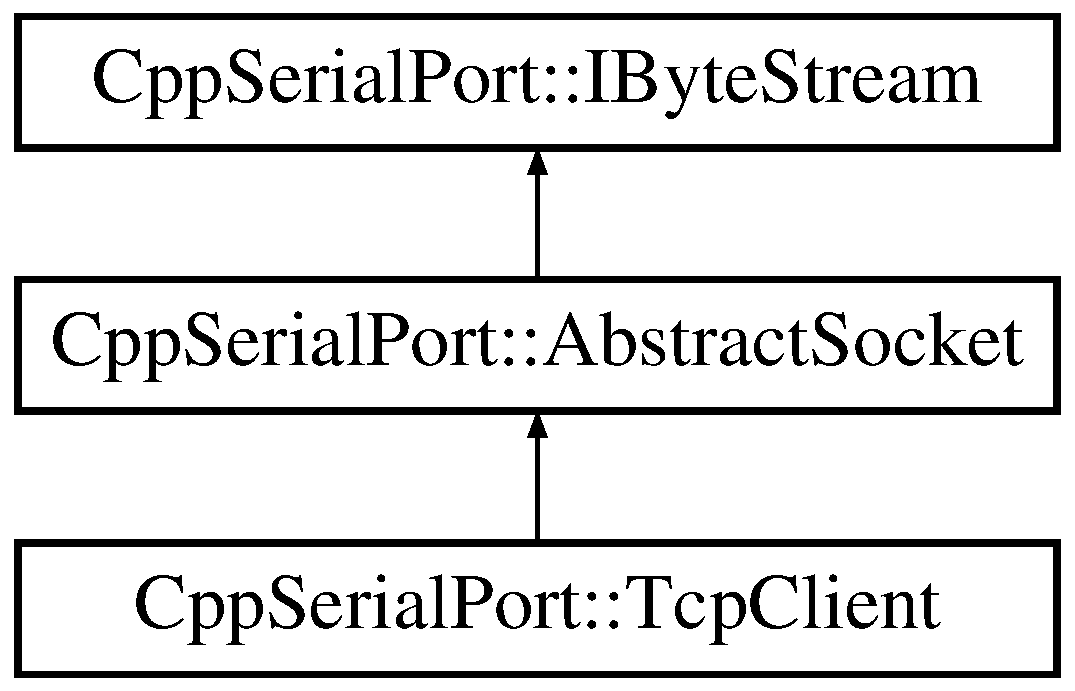
\includegraphics[height=3.000000cm]{class_cpp_serial_port_1_1_tcp_client}
\end{center}
\end{figure}
\subsection*{Public Member Functions}
\begin{DoxyCompactItemize}
\item 
\mbox{\Hypertarget{class_cpp_serial_port_1_1_tcp_client_af0919ce0261dcb67d8d23ba25f052a00}\label{class_cpp_serial_port_1_1_tcp_client_af0919ce0261dcb67d8d23ba25f052a00}} 
{\bfseries Tcp\+Client} (const std\+::string \&host\+Name, uint16\+\_\+t port\+Number)
\item 
\mbox{\Hypertarget{class_cpp_serial_port_1_1_tcp_client_a98ff90e57b266dcd1416da536ad0e317}\label{class_cpp_serial_port_1_1_tcp_client_a98ff90e57b266dcd1416da536ad0e317}} 
{\bfseries Tcp\+Client} (const \mbox{\hyperlink{class_cpp_serial_port_1_1_i_p_v4_address}{I\+P\+V4\+Address}} \&ip\+Address, uint16\+\_\+t port\+Number)
\end{DoxyCompactItemize}
\subsection*{Protected Member Functions}
\begin{DoxyCompactItemize}
\item 
\mbox{\Hypertarget{class_cpp_serial_port_1_1_tcp_client_a2f8828127e62cd21e760624c9bd32311}\label{class_cpp_serial_port_1_1_tcp_client_a2f8828127e62cd21e760624c9bd32311}} 
ssize\+\_\+t {\bfseries do\+Write} (const char $\ast$bytes, size\+\_\+t byte\+Count) override
\item 
\mbox{\Hypertarget{class_cpp_serial_port_1_1_tcp_client_a35ce6d6bd181cd586863d0a7f7f48f5c}\label{class_cpp_serial_port_1_1_tcp_client_a35ce6d6bd181cd586863d0a7f7f48f5c}} 
ssize\+\_\+t {\bfseries do\+Read} (char $\ast$buffer, size\+\_\+t buffer\+Max) override
\item 
\mbox{\Hypertarget{class_cpp_serial_port_1_1_tcp_client_aec9df600c145f1456e3b0ceb4374077d}\label{class_cpp_serial_port_1_1_tcp_client_aec9df600c145f1456e3b0ceb4374077d}} 
void {\bfseries do\+Connect} (addrinfo $\ast$address\+Info) override
\item 
\mbox{\Hypertarget{class_cpp_serial_port_1_1_tcp_client_a4d5e2349357b375bf1ff88ea409fa574}\label{class_cpp_serial_port_1_1_tcp_client_a4d5e2349357b375bf1ff88ea409fa574}} 
addrinfo {\bfseries get\+Address\+Info\+Hints} () override
\end{DoxyCompactItemize}
\subsection*{Additional Inherited Members}


The documentation for this class was generated from the following files\+:\begin{DoxyCompactItemize}
\item 
Cpp\+Serial\+Port/Tcp\+Client.\+h\item 
Cpp\+Serial\+Port/Tcp\+Client.\+cpp\end{DoxyCompactItemize}

\hypertarget{class_cpp_serial_port_1_1_udp_client}{}\section{Cpp\+Serial\+Port\+:\+:Udp\+Client Class Reference}
\label{class_cpp_serial_port_1_1_udp_client}\index{Cpp\+Serial\+Port\+::\+Udp\+Client@{Cpp\+Serial\+Port\+::\+Udp\+Client}}
Inheritance diagram for Cpp\+Serial\+Port\+:\+:Udp\+Client\+:\begin{figure}[H]
\begin{center}
\leavevmode
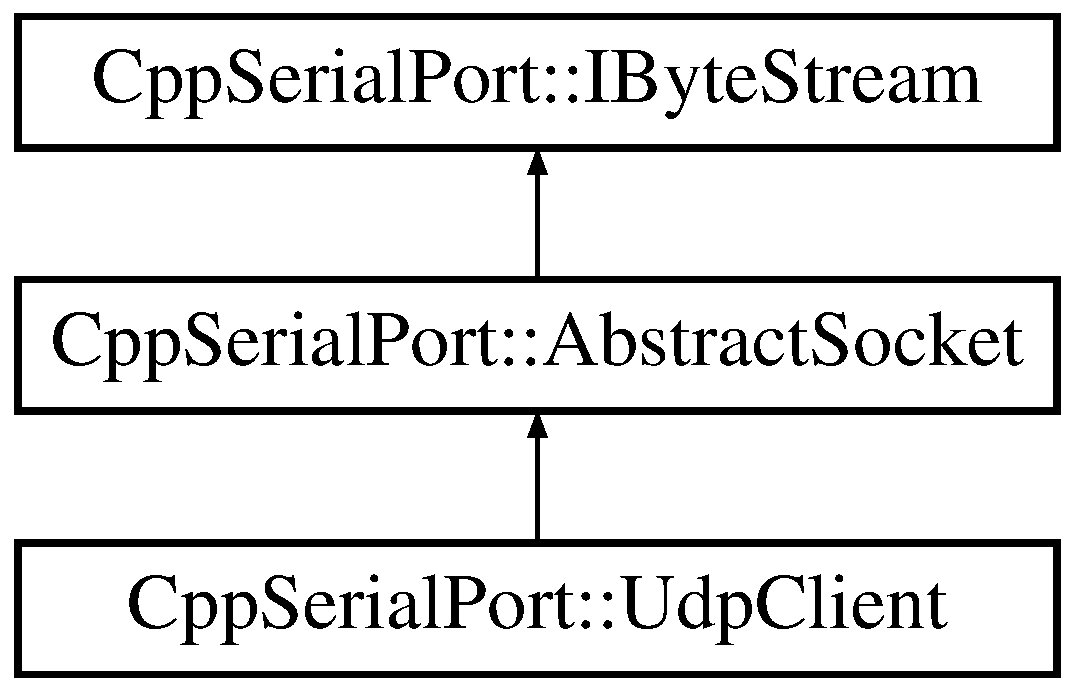
\includegraphics[height=3.000000cm]{class_cpp_serial_port_1_1_udp_client}
\end{center}
\end{figure}
\subsection*{Public Member Functions}
\begin{DoxyCompactItemize}
\item 
\mbox{\Hypertarget{class_cpp_serial_port_1_1_udp_client_aad37324f9f4581da620574c31ea0bc46}\label{class_cpp_serial_port_1_1_udp_client_aad37324f9f4581da620574c31ea0bc46}} 
{\bfseries Udp\+Client} (const std\+::string \&host\+Name, uint16\+\_\+t port\+Number)
\item 
\mbox{\Hypertarget{class_cpp_serial_port_1_1_udp_client_abaf921b2a2ea9541a8ead4b812fcae36}\label{class_cpp_serial_port_1_1_udp_client_abaf921b2a2ea9541a8ead4b812fcae36}} 
{\bfseries Udp\+Client} (const \mbox{\hyperlink{class_cpp_serial_port_1_1_i_p_v4_address}{I\+P\+V4\+Address}} \&ip\+Address, uint16\+\_\+t port\+Number)
\end{DoxyCompactItemize}
\subsection*{Protected Member Functions}
\begin{DoxyCompactItemize}
\item 
\mbox{\Hypertarget{class_cpp_serial_port_1_1_udp_client_ac383e76251afd149db2dd3b26d649bcd}\label{class_cpp_serial_port_1_1_udp_client_ac383e76251afd149db2dd3b26d649bcd}} 
ssize\+\_\+t {\bfseries do\+Write} (const char $\ast$bytes, size\+\_\+t byte\+Count) override
\item 
\mbox{\Hypertarget{class_cpp_serial_port_1_1_udp_client_ad0952d23227c989886903a5d711ee2c9}\label{class_cpp_serial_port_1_1_udp_client_ad0952d23227c989886903a5d711ee2c9}} 
ssize\+\_\+t {\bfseries do\+Read} (char $\ast$buffer, size\+\_\+t buffer\+Max) override
\item 
\mbox{\Hypertarget{class_cpp_serial_port_1_1_udp_client_acf4d84370ebc9e7ca70e77ad79123efa}\label{class_cpp_serial_port_1_1_udp_client_acf4d84370ebc9e7ca70e77ad79123efa}} 
void {\bfseries do\+Connect} (addrinfo $\ast$address\+Info) override
\item 
\mbox{\Hypertarget{class_cpp_serial_port_1_1_udp_client_a72269903ffd7d1b3d6c8b487af4ab6ed}\label{class_cpp_serial_port_1_1_udp_client_a72269903ffd7d1b3d6c8b487af4ab6ed}} 
addrinfo {\bfseries get\+Address\+Info\+Hints} () override
\end{DoxyCompactItemize}
\subsection*{Additional Inherited Members}


The documentation for this class was generated from the following files\+:\begin{DoxyCompactItemize}
\item 
Cpp\+Serial\+Port/Udp\+Client.\+h\item 
Cpp\+Serial\+Port/Udp\+Client.\+cpp\end{DoxyCompactItemize}

\hypertarget{union_cpp_serial_port_1_1_underlying_bytes}{}\section{Cpp\+Serial\+Port\+:\+:Underlying\+Bytes Union Reference}
\label{union_cpp_serial_port_1_1_underlying_bytes}\index{Cpp\+Serial\+Port\+::\+Underlying\+Bytes@{Cpp\+Serial\+Port\+::\+Underlying\+Bytes}}
\subsection*{Public Attributes}
\begin{DoxyCompactItemize}
\item 
\mbox{\Hypertarget{union_cpp_serial_port_1_1_underlying_bytes_afc39c8526c0656fc0d04299782d0c431}\label{union_cpp_serial_port_1_1_underlying_bytes_afc39c8526c0656fc0d04299782d0c431}} 
uint32\+\_\+t {\bfseries address}
\item 
\mbox{\Hypertarget{union_cpp_serial_port_1_1_underlying_bytes_a32fff31872b18ddf0750ce09243c5a93}\label{union_cpp_serial_port_1_1_underlying_bytes_a32fff31872b18ddf0750ce09243c5a93}} 
uint8\+\_\+t {\bfseries bytes} \mbox{[}sizeof(uint32\+\_\+t)\mbox{]}
\end{DoxyCompactItemize}


The documentation for this union was generated from the following file\+:\begin{DoxyCompactItemize}
\item 
Cpp\+Serial\+Port/I\+P\+V4\+Address.\+h\end{DoxyCompactItemize}

%--- End generated contents ---

% Index
\backmatter
\newpage
\phantomsection
\clearemptydoublepage
\addcontentsline{toc}{chapter}{Index}
\printindex

\end{document}
